% !TEX program = xelatex %指定编译方式xelatex。
% !BIB program = biber %指定bib数据后台处理程序biber。
\documentclass[11pt,a4paper,UTF8,titlepage]{ctexrep} %指定ctex的文档类,设置基本字号为11pt,a4大小,使用UTF-8编码保存,指定\maketitle生成单独的标题页。

\usepackage{syntonly}
%\syntaxonly %用来快速编译以排查错误,不生成DVI或PDF。
\usepackage[style=gb7714-2015]{biblatex} %调用biblatex宏包,设置参考文献样式(符合中文文献著录标准GB/T 7714-2015的样式),使用默认的后端程序biber(其支持更好,包括UTF-8等)放弃使用[backend=bibtex](只支持ascii编码)。
\addbibresource{resources/reference.bib} %加载参考文献数据库。
\usepackage{makeidx}
\makeindex %开启索引收集
\usepackage[margin=1in]{geometry} %调用geometry宏包,设置周围页边距为1英寸(为电子档设计,非打印)。
\usepackage{xcolor} %调用xcolor宏包,以支持扩展生成颜色。
\usepackage{fontspec} %调用fontspec宏包以更改西文字体族。
\setmainfont{Source Serif Pro}
\setsansfont{Source Sans Pro}
\setmonofont{Source Code Pro}
\usepackage{xeCJK} %调用xeCJK宏包以更改中文字体族。
\xeCJKsetup{AutoFakeSlant=true}  %设置xeCJK选项-伪斜体(需置于字体设置之前)。
\setCJKmainfont{思源宋体}
\setCJKsansfont{思源黑体}
\setCJKmonofont{思源等宽}
\usepackage{graphicx} %调用graphicx宏包,以支持插图。
\graphicspath{{resources/images/},{resources/images/FollowMe/}} %加载图片路径。
\usepackage{caption} %调用caption,支持不带编号的标题。
\usepackage{wrapfig} %调用wrapfig,支持图文排版。
\usepackage{subfigure} %调用subfigure宏包进行图片图片排版。
\usepackage{tikz,tikz-qtree} %调用tikz及其扩展宏包,以支持画图。
\usepackage[subfigure]{tocloft} %tocloft与subfigure宏包冲突,不能简单调用,tocloft需设置参数。
\usepackage{tocbibind} %调用宏包以添加目录本身和参考文献进目录中。
\usepackage{multicol} %调用multicol宏包以支持多栏排版。
\usepackage[toc]{multitoc} %调用multitoc宏包,设置toc目录页,默认双栏排版。
\usepackage{enumitem} %调用emuitem,以设置列表环境。
\usepackage{multirow} %调用multirow,以支持纵向合并列表。
\setlist{left=0em}
%重订制目录命令。
\renewcommand{\tableofcontents}%
  {\chapter{\contentsname}%
  \@mkboth{\MakeUppercase\contentsname}{\MakeUppercase\contentsname}%
  \@makeschapterhead{\sourcecodename}%
  \@starttoc{toc}%
}
\usepackage{fancyhdr} %调用宏包,以设置页眉,统一格式:标题在左,页码在右。
\pagestyle{fancy}
\fancyhf{}
\fancyhead[LO]{\sffamily \rightmark}
\fancyhead[LE]{\sffamily \leftmark}
\fancyhead[ROE]{\bfseries \thepage}
\fancyfoot[COE]{\ttfamily \href{https://mister-kin.github.io}{个人博客:https://mister-kin.github.io}}
%定义intro环境。
\newenvironment{intro}{\narrower\sffamily}{\par\vspace*{2ex plus 2.5ex minus 1.5ex}}
\usepackage{listings} % 指定listings,订制代码排版环境
\lstset{
    basicstyle      = \ttfamily,                          % 基本代码指定等宽字体
    keywordstyle    = \bfseries,                          % 关键字指定加粗
    commentstyle    = \ttfamily\slshape\color{gray},      % 注释指定灰色等宽斜体
    stringstyle     = \ttfamily,                          % 字符串指定等宽字体
    %numbers        = left,                               % 行号的位置在左边,启用后不方便复制代码
    %numberstyle    = \ttfamily,                          % 行号等宽字体
    %xleftmargin    = \parindent,                         % 代码左边框起始位置(启用行号时建议启用这个)
    %frame          = trBL,                               % 代码框类型,t下,r右,b下,l左,大写时为两条线。
    %frameround     = fttt,                               % 控制代码框是否为圆角
    frameshape      = {{ryrynyyyy}{yny}{yny}{ryrynyyyy}}, % 控制边框样式,上下边是每三个字母段控制一条边框。
    backgroundcolor = \color{gray!5},                     % 代码框背景颜色:5%的灰色
    breaklines      = true,                               % 代码过长时则换行
    gobble          = 8,                                  % 去掉代码前的缩进
}
\usepackage{hyperref} %调用hyperref宏包
\hypersetup{
    colorlinks=true, %设置超链接文件带颜色
    bookmarks=true, %生成书签
    bookmarksopen=true, %书签展开
    bookmarksnumbered=true, %书签带章节编号
    CJKbookmarks=true, %cjk必设参数
    unicode, %utf-8编码必设参数
    pdftitle=英语学习笔记, %设置PDF文件属性标题
    pdfauthor=Mr. Kin, %设置PDF文件属性作者
    pdfstartview=FitH %默认适合宽度显示
}

\newcommand{\collections} % 定义汇总文件命令,以方便拆分源文件进行编写。

    \title{\hypertarget{title}{\textbf{英语学习笔记}}}
    \addcontentsline{toc}{chapter}{标题页}
    \author{Written by Mr. Kin}
    \date{创建于2020.2.12,修改于\number\year.\number\month.\number\day}

\begin{document}
    \phantomsection %确保目录中的超链接指向正确的页码
    \pdfbookmark[1]{标题页}{title} %添加标题页书签
    \pagenumbering{Roman} %大写罗马样式页码
    \maketitle %生成标题页
    \pagenumbering{roman} %小写罗马样式页码
    % !TEX root = OneClickSwitchLanguage.tex %指定主文件。
\ifx\collections\undefined
% !TEX program = xelatex %指定编译方式xelatex。
% !BIB program = biber %指定bib数据后台处理程序biber。
\documentclass[11pt,a4paper,UTF8,titlepage]{ctexart} %指定ctexart文档类,设置基本字号为11pt,a4大小,使用UTF-8编码保存,指定\maketitle生成单独的标题页。

\usepackage{syntonly}
%\syntaxonly %用来快速编译以排查错误,不生成DVI或PDF。
\usepackage[style=gb7714-2015]{biblatex} %调用biblatex宏包,设置参考文献样式(符合中文文献著录标准GB/T 7714-2015的样式),使用默认的后端程序biber(其支持更好,包括UTF-8等)放弃使用[backend=bibtex](只支持ascii编码)。
\addbibresource{resources/reference.bib} %加载参考文献数据库。
\usepackage{makeidx}
\makeindex %开启索引收集
\usepackage[margin=1in]{geometry} %调用geometry宏包,设置周围页边距为1英寸(为电子档设计,非打印)。
\usepackage{xcolor} %调用xcolor宏包,以支持扩展生成颜色。
\usepackage{fontspec} %调用fontspec宏包以更改西文字体族。
\setmainfont{Source Serif Pro}
\setsansfont{Source Sans Pro}
\setmonofont{Source Code Pro}
\usepackage{xeCJK} %调用xeCJK宏包以更改中文字体族。
\xeCJKsetup{AutoFakeSlant=true}  %设置xeCJK选项-伪斜体(需置于字体设置之前)。
\setCJKmainfont{思源宋体}
\setCJKsansfont{思源黑体}
\setCJKmonofont{思源等宽}
\usepackage{graphicx} %调用graphicx宏包,以支持插图。
\graphicspath{{resources/images/},{resources/images/FollowMe/}} %加载图片路径。
\usepackage{caption} %调用caption,支持不带编号的标题。
\usepackage{wrapfig} %调用wrapfig,支持图文排版。
\usepackage{subfigure} %调用subfigure宏包进行图片图片排版。
\usepackage{tikz,tikz-qtree} %调用tikz及其扩展宏包,以支持画图。
\usepackage[subfigure]{tocloft} %tocloft与subfigure宏包冲突,不能简单调用,tocloft需设置参数。
\usepackage{tocbibind} %调用宏包以添加目录本身和参考文献进目录中。
\usepackage{multicol} %调用multicol宏包以支持多栏排版。
\usepackage[toc]{multitoc} %调用multitoc宏包,设置toc目录页,默认双栏排版。
\usepackage{enumitem} %调用emuitem,以设置列表环境。
\usepackage{multirow} %调用multirow,以支持纵向合并列表。
%重订制目录命令。
\renewcommand{\tableofcontents}%
  {\chapter{\contentsname}%
  \@mkboth{\MakeUppercase\contentsname}{\MakeUppercase\contentsname}%
  \@makeschapterhead{\sourcecodename}%
  \@starttoc{toc}%
}
\usepackage{fancyhdr} %调用宏包,以设置页眉,统一格式:标题在左,页码在右。
\pagestyle{fancy}
\fancyhf{}
\fancyhead[LO]{\sffamily \rightmark}
\fancyhead[LE]{\sffamily \leftmark}
\fancyhead[ROE]{\bfseries \thepage}
\fancyfoot[COE]{\ttfamily \href{https://mister-kin.github.io}{个人博客:https://mister-kin.github.io}}
%定义intro环境。
\newenvironment{intro}{\narrower\sffamily}{\par\vspace*{2ex plus 2.5ex minus 1.5ex}}
\usepackage{listings} % 指定listings,订制代码排版环境
\lstset{
    basicstyle      = \ttfamily,                          % 基本代码指定等宽字体
    keywordstyle    = \bfseries,                          % 关键字指定加粗
    commentstyle    = \ttfamily\slshape\color{gray},      % 注释指定灰色等宽斜体
    stringstyle     = \ttfamily,                          % 字符串指定等宽字体
    %numbers        = left,                               % 行号的位置在左边,启用后不方便复制代码
    %numberstyle    = \ttfamily,                          % 行号等宽字体
    %xleftmargin    = \parindent,                         % 代码左边框起始位置(启用行号时建议启用这个)
    %frame          = trBL,                               % 代码框类型,t下,r右,b下,l左,大写时为两条线。
    %frameround     = fttt,                               % 控制代码框是否为圆角
    frameshape      = {{ryrynyyyy}{yny}{yny}{ryrynyyyy}}, % 控制边框样式,上下边是每三个字母段控制一条边框。
    backgroundcolor = \color{gray!5},                     % 代码框背景颜色:5%的灰色
    breaklines      = true,                               % 代码过长时则换行
    gobble          = 8,                                  % 去掉代码前的缩进
}
\usepackage{hyperref} %调用hyperref宏包
\hypersetup{
    colorlinks=true, %设置超链接文件带颜色
    bookmarks=true, %生成书签
    bookmarksopen=true, %书签展开
    bookmarksnumbered=true, %书签带章节编号
    CJKbookmarks=true, %cjk必设参数
    unicode, %utf-8编码必设参数
    pdftitle=标题, %设置PDF文件属性标题
    pdfauthor=Mr. Kin, %设置PDF文件属性作者
    pdfstartview=FitH %默认适合宽度显示
}

    \title{\hypertarget{title}{\textbf{标题}}}
    \addcontentsline{toc}{section}{标题页}
    \author{Written by Mr. Kin}
    \date{创建于2020.6.7,修改于\number\year.\number\month.\number\day}

\begin{document}
    \phantomsection %确保目录中的超链接指向正确的页码
    \pdfbookmark[1]{标题页}{title} %添加标题页书签
    \pagenumbering{Roman} %大写罗马样式页码
    \maketitle %生成标题页
    \pagenumbering{roman} %小写罗马样式页码
    {\centering \tableofcontents} %生成目录页
    \clearpage %新建页,分离上下两个样式页码的效果
    \pagenumbering{arabic} %阿拉伯样式页码
    \fi

    \phantomsection
    \section*{\bfseries \sffamily 关于作者}
    \addcontentsline{toc}{section}{关于作者}
    \markright{关于作者}

    \subsection*{\bfseries \sffamily 关于我}
    \begin{wrapfigure}[3]{L}{60pt}
        \vspace*{-20pt}
        \centering
        
\includegraphics{kin-logo}
    \end{wrapfigure}
    Mr. Kin,广东客家仁,程序猿,CG和游戏爱好者,一枚极客学生党。B站翻译up,个人up。不定时在B站直播日常:码代码,码博客,翻译,做视频,做教程。 ($\vartheta$$\bullet$\_$\bullet$)$\vartheta$ \hyperlink{follow}{\emph{(点击关注我!)}}

    \subsection*{\bfseries \sffamily 开源建设}

    \noindent 参与的开源软件中文化翻译

    \begin{itemize}
        \item krita文档:2018.8.5 - 2019.4.23
        \item \href{https://www.blendercn.org/5812.html?tdsourcetag=s_pctim_aiomsg}{Blender手册}:2019.7.20 - 2019.9.4 - 至今(\href{https://developer.blender.org/p/Mr_Kin/}{翻译维护})
    \end{itemize}

    \subsection*{\bfseries \sffamily \hypertarget{contact}{联系方式}}
    \vspace*{-1ex}
    \noindent {\footnotesize \emph{\color{red}注:联系时请注明身份,谢谢!}}

    \begin{itemize}
        \item QQ:\href{tencent://AddContact/?fromId=45&fromSubId=1&subcmd=all&uin=2312463626&website=www.oicqzone.com}{2312463626}\emph{\color{red}(点击号码加好友)}
        \item 邮箱:2312463626@qq.com ;moyu1355@gmail.com
    \end{itemize}

    \subsection*{\bfseries \sffamily \hypertarget{follow}{关注渠道}}
    \vspace*{-1ex}
    \noindent {\footnotesize\emph{\color{red}注:点击文字即可跳转关注!}}
    \vspace*{-2ex}

    \begin{figure}[htbp]
        \centering
        
\includegraphics[scale=0.2]{WechatOfficialAccounts.png}
    \end{figure}
    \vspace*{-4ex}

    \begin{figure}[htbp]
        \centering
        \begin{minipage}[t]{0.2\textwidth}
            \centering
            \setlength{\abovecaptionskip}{1pt}
            \caption*{\href{https://mister-kin.github.io}{博客 - Blog}}
            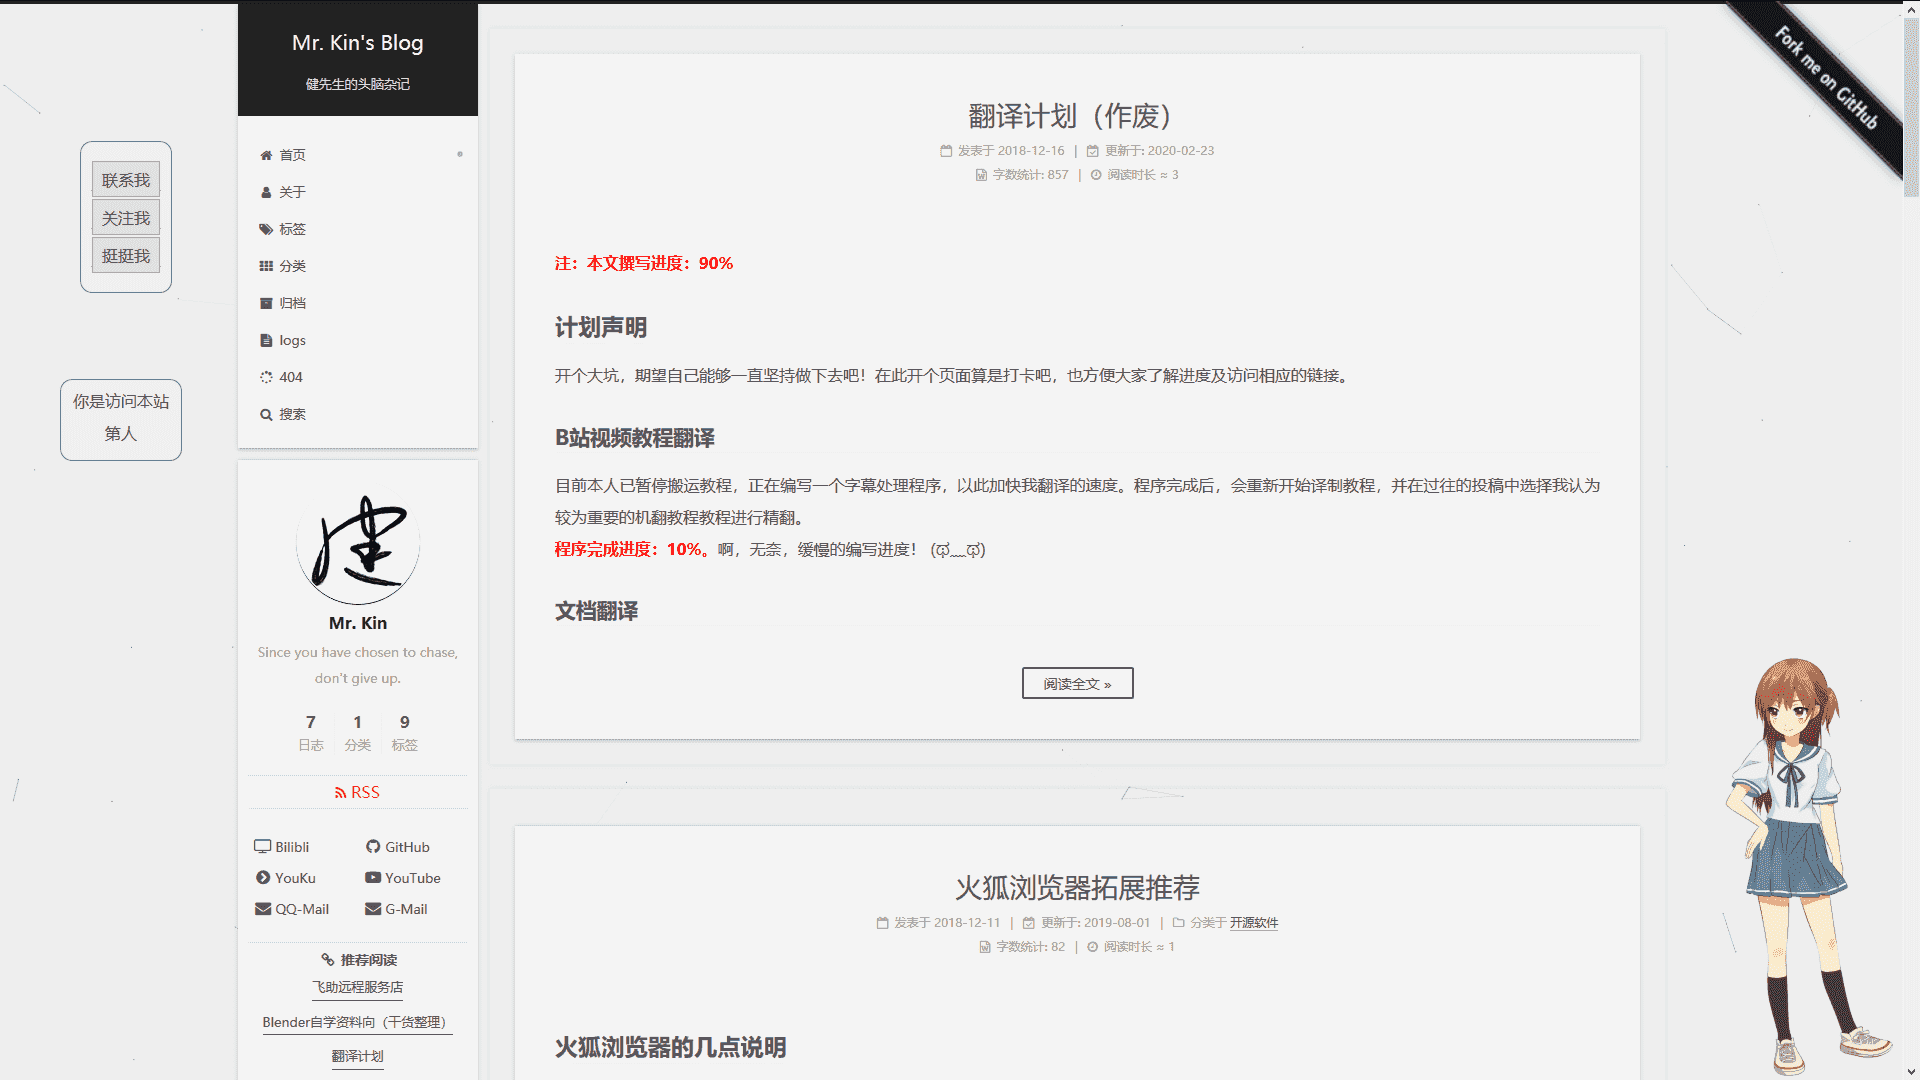
\includegraphics[scale=0.055]{Blog}
        \end{minipage}
        \qquad
        \begin{minipage}[t]{0.2\textwidth}
            \centering
            \setlength{\abovecaptionskip}{1pt}
            \caption*{\href{https://github.com/mister-kin}{Github}}
            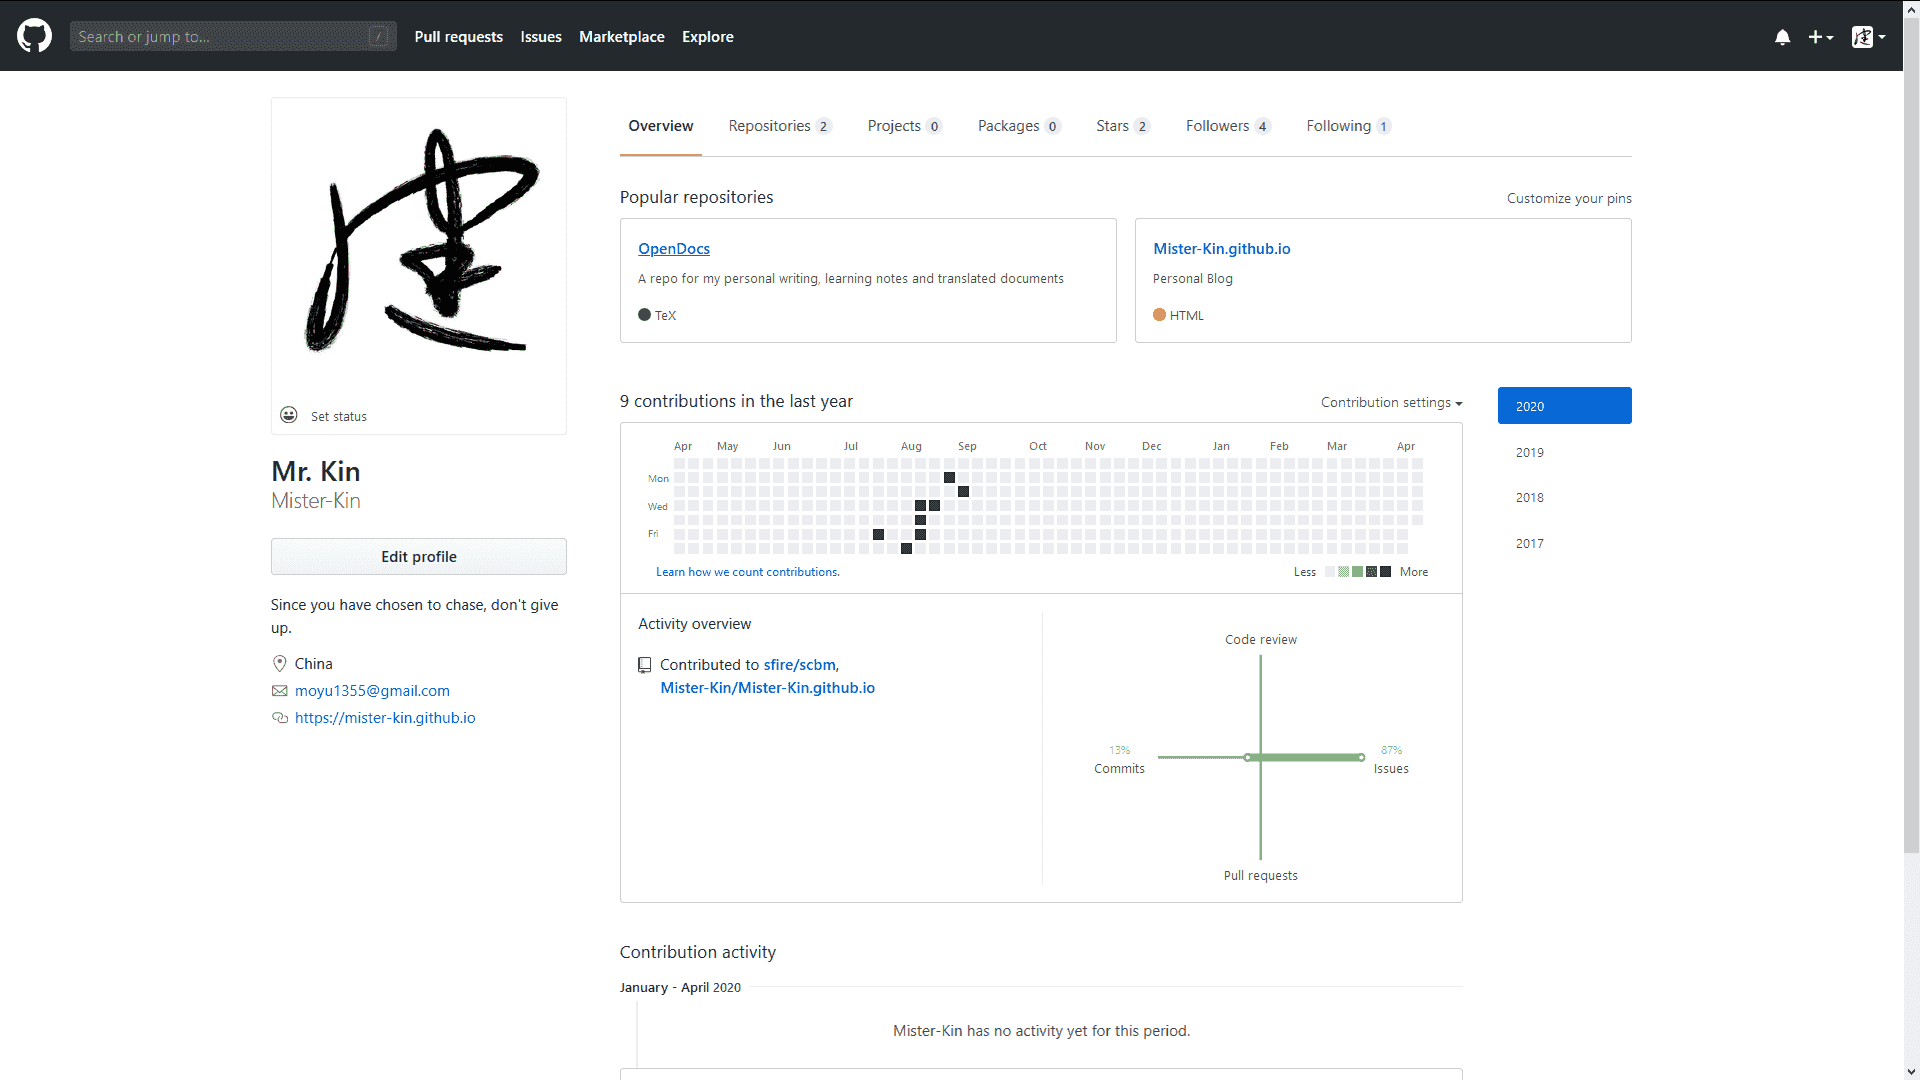
\includegraphics[scale=0.055]{Github}
        \end{minipage}
        \qquad
        \begin{minipage}[t]{0.2\textwidth}
            \centering
            \setlength{\abovecaptionskip}{1pt}
            \caption*{\href{https://weibo.com/6270111192/profile?topnav=1&wvr=6&is_all=1}{微博 - Weibo}}
            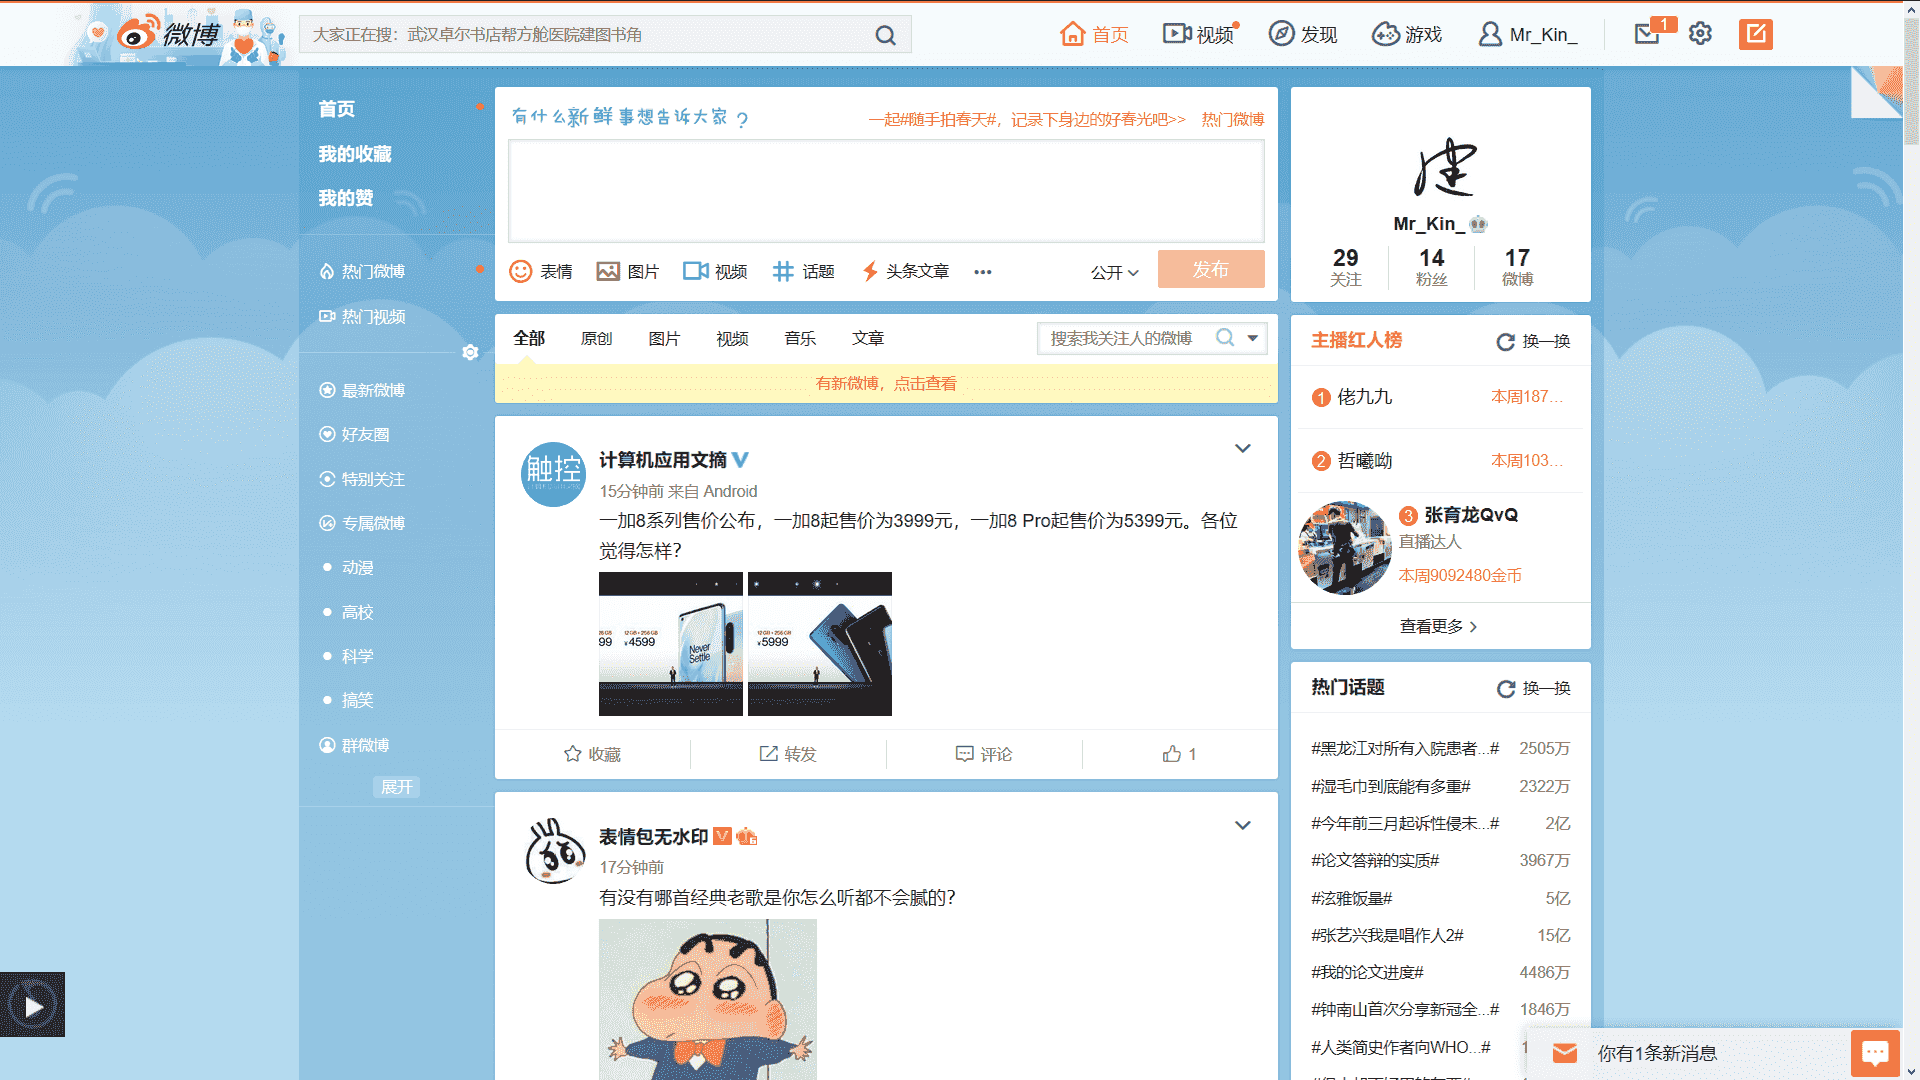
\includegraphics[scale=0.055]{Weibo}
        \end{minipage}
        \qquad
        \begin{minipage}[t]{0.2\textwidth}
            \centering
            \setlength{\abovecaptionskip}{1pt}
            \caption*{\href{https://www.zhihu.com/people/drwu-94}{知乎 - Zhihu}}
            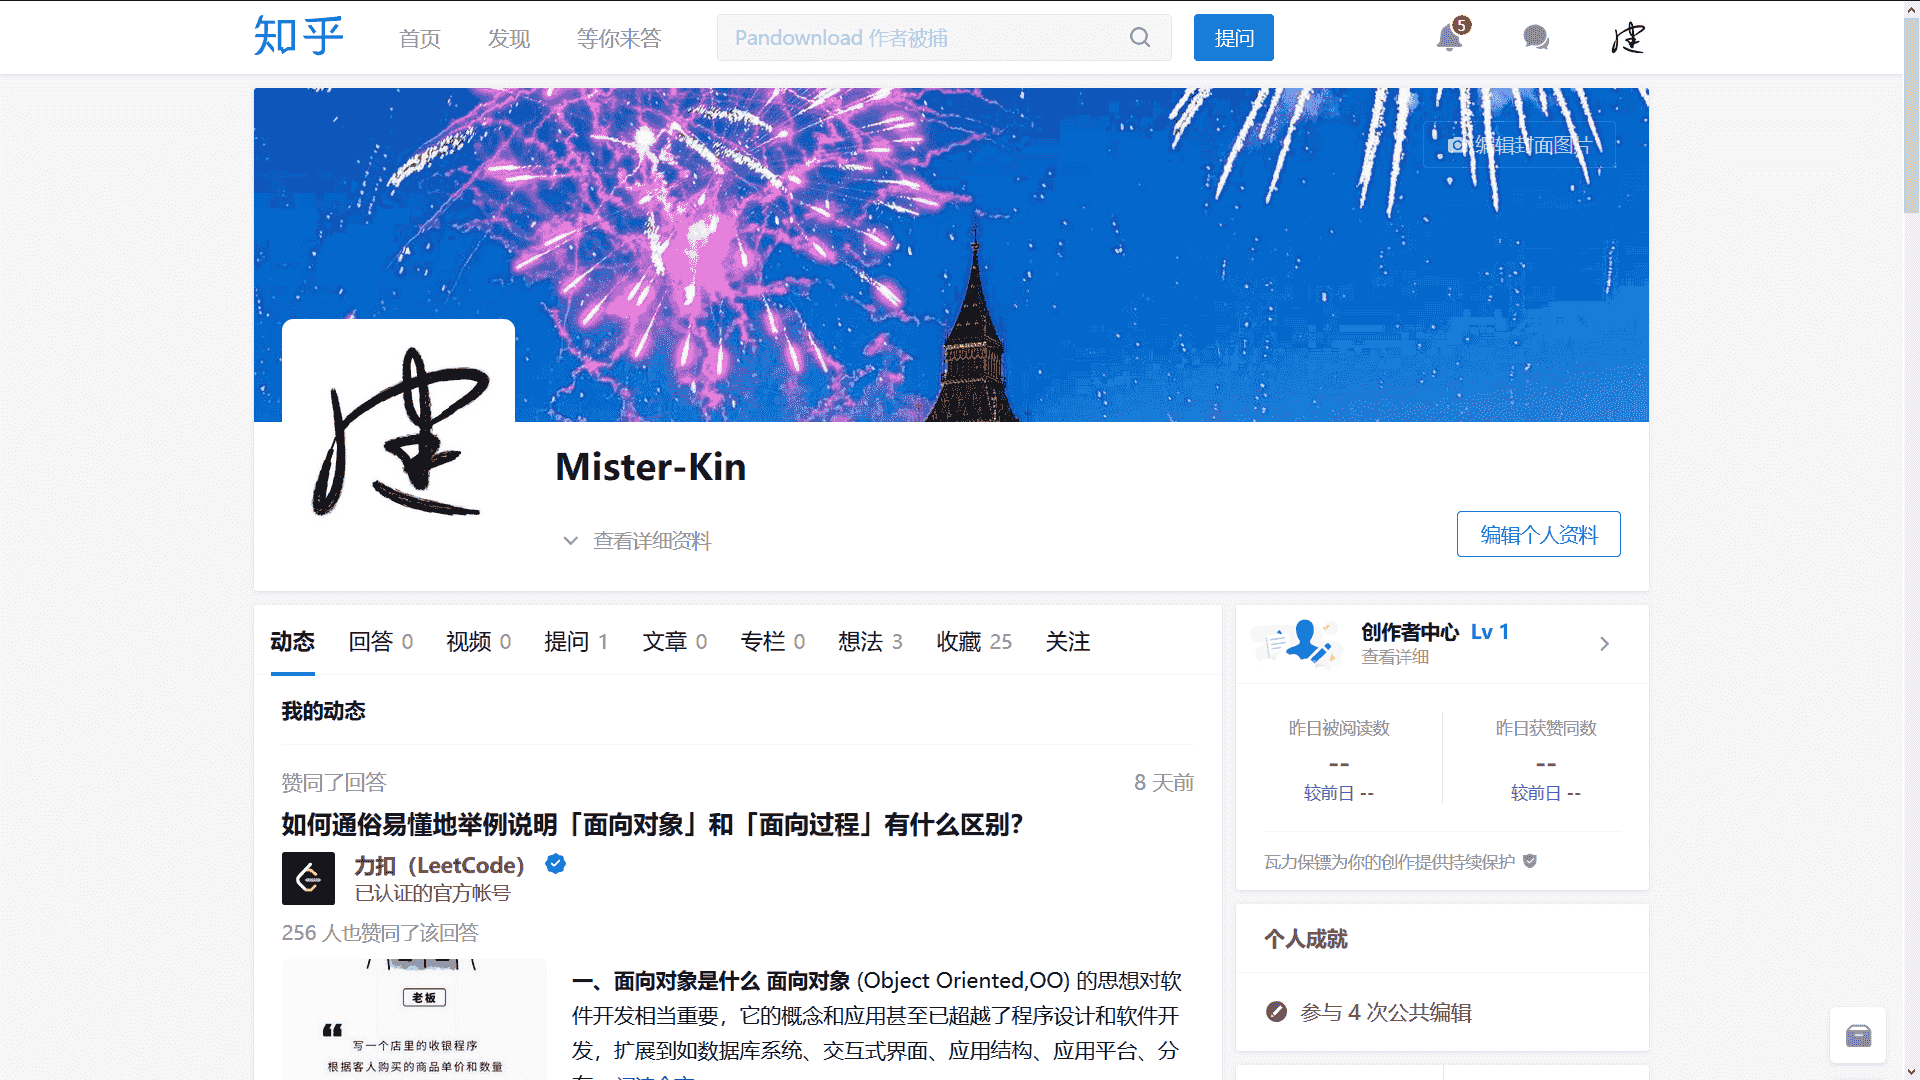
\includegraphics[scale=0.055]{Zhihu}
        \end{minipage}
        \qquad

        \begin{minipage}[t]{0.2\textwidth}
            \centering
            \setlength{\abovecaptionskip}{1pt}
            \setlength{\belowcaptionskip}{10pt}
            \caption*{\href{http://space.bilibili.com/17025250?}{B站 - Bilibili}}
            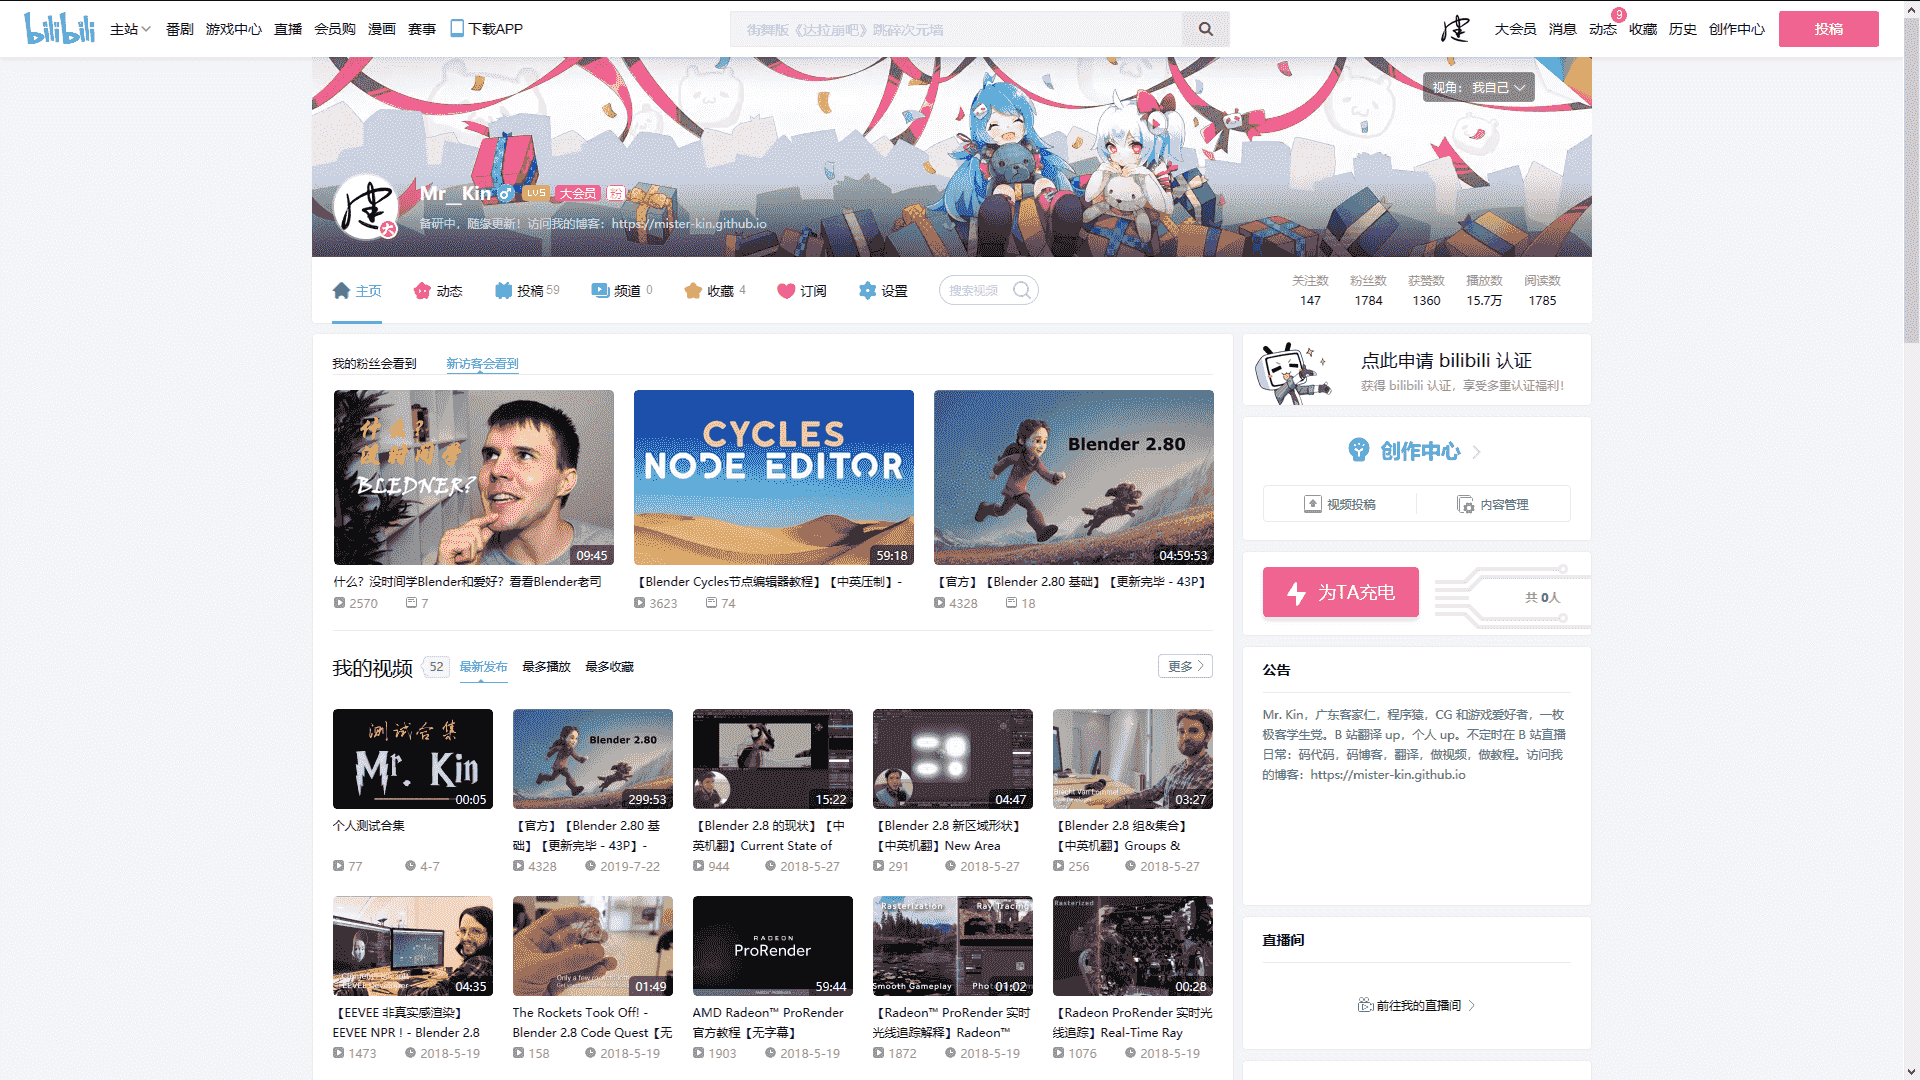
\includegraphics[scale=0.055]{Bilibili}
        \end{minipage}
        \qquad
        \begin{minipage}[t]{0.2\textwidth}
            \centering
            \setlength{\abovecaptionskip}{1pt}
            \setlength{\belowcaptionskip}{10pt}
            \caption*{\href{http://i.youku.com/i/UNjA3MTk5Mjgw?spm=a2hzp.8253869.0.0}{优酷 - Youku}}
            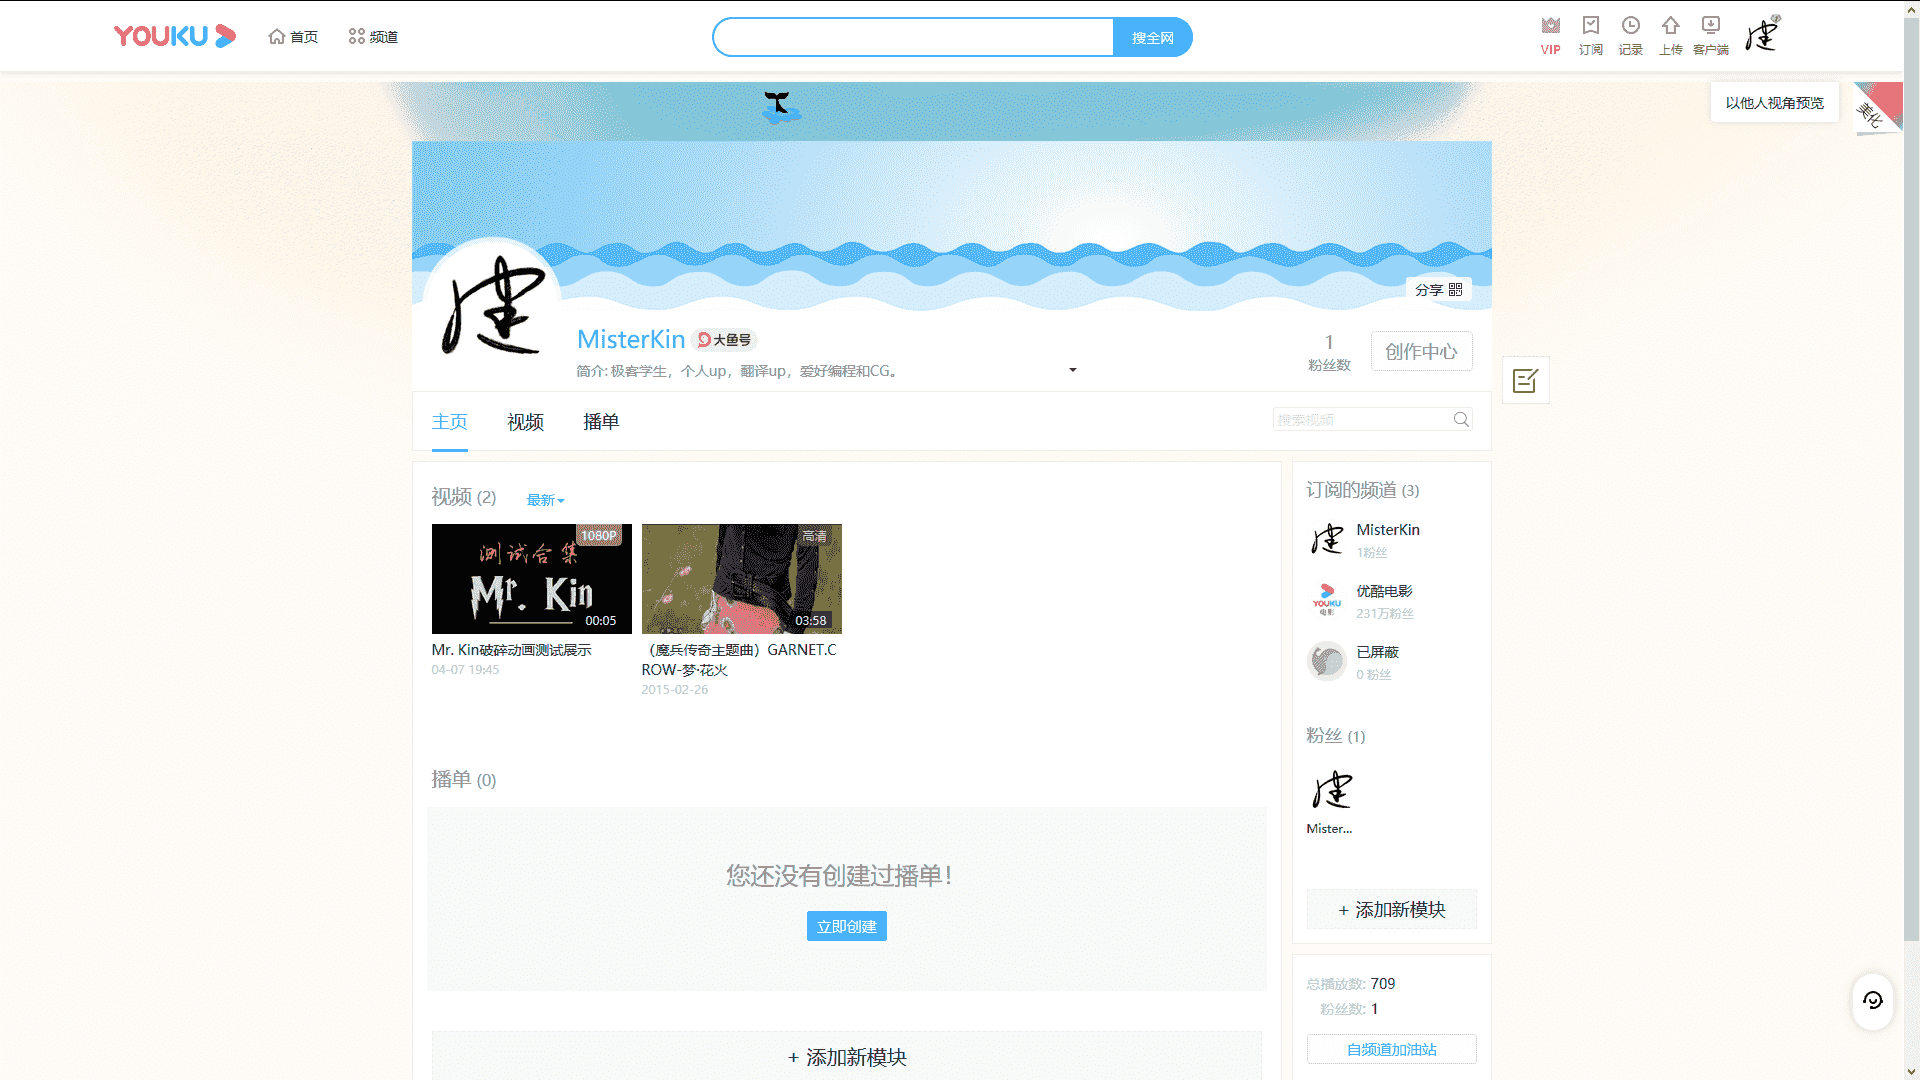
\includegraphics[scale=0.055]{Youku}
        \end{minipage}
        \qquad
        \begin{minipage}[t]{0.2\textwidth}
            \centering
            \setlength{\abovecaptionskip}{1pt}
            \setlength{\belowcaptionskip}{10pt}
            \caption*{\href{https://www.toutiao.com/c/user/835254071079053/\#mid=1663279303982091}{头条 - Headline}}
            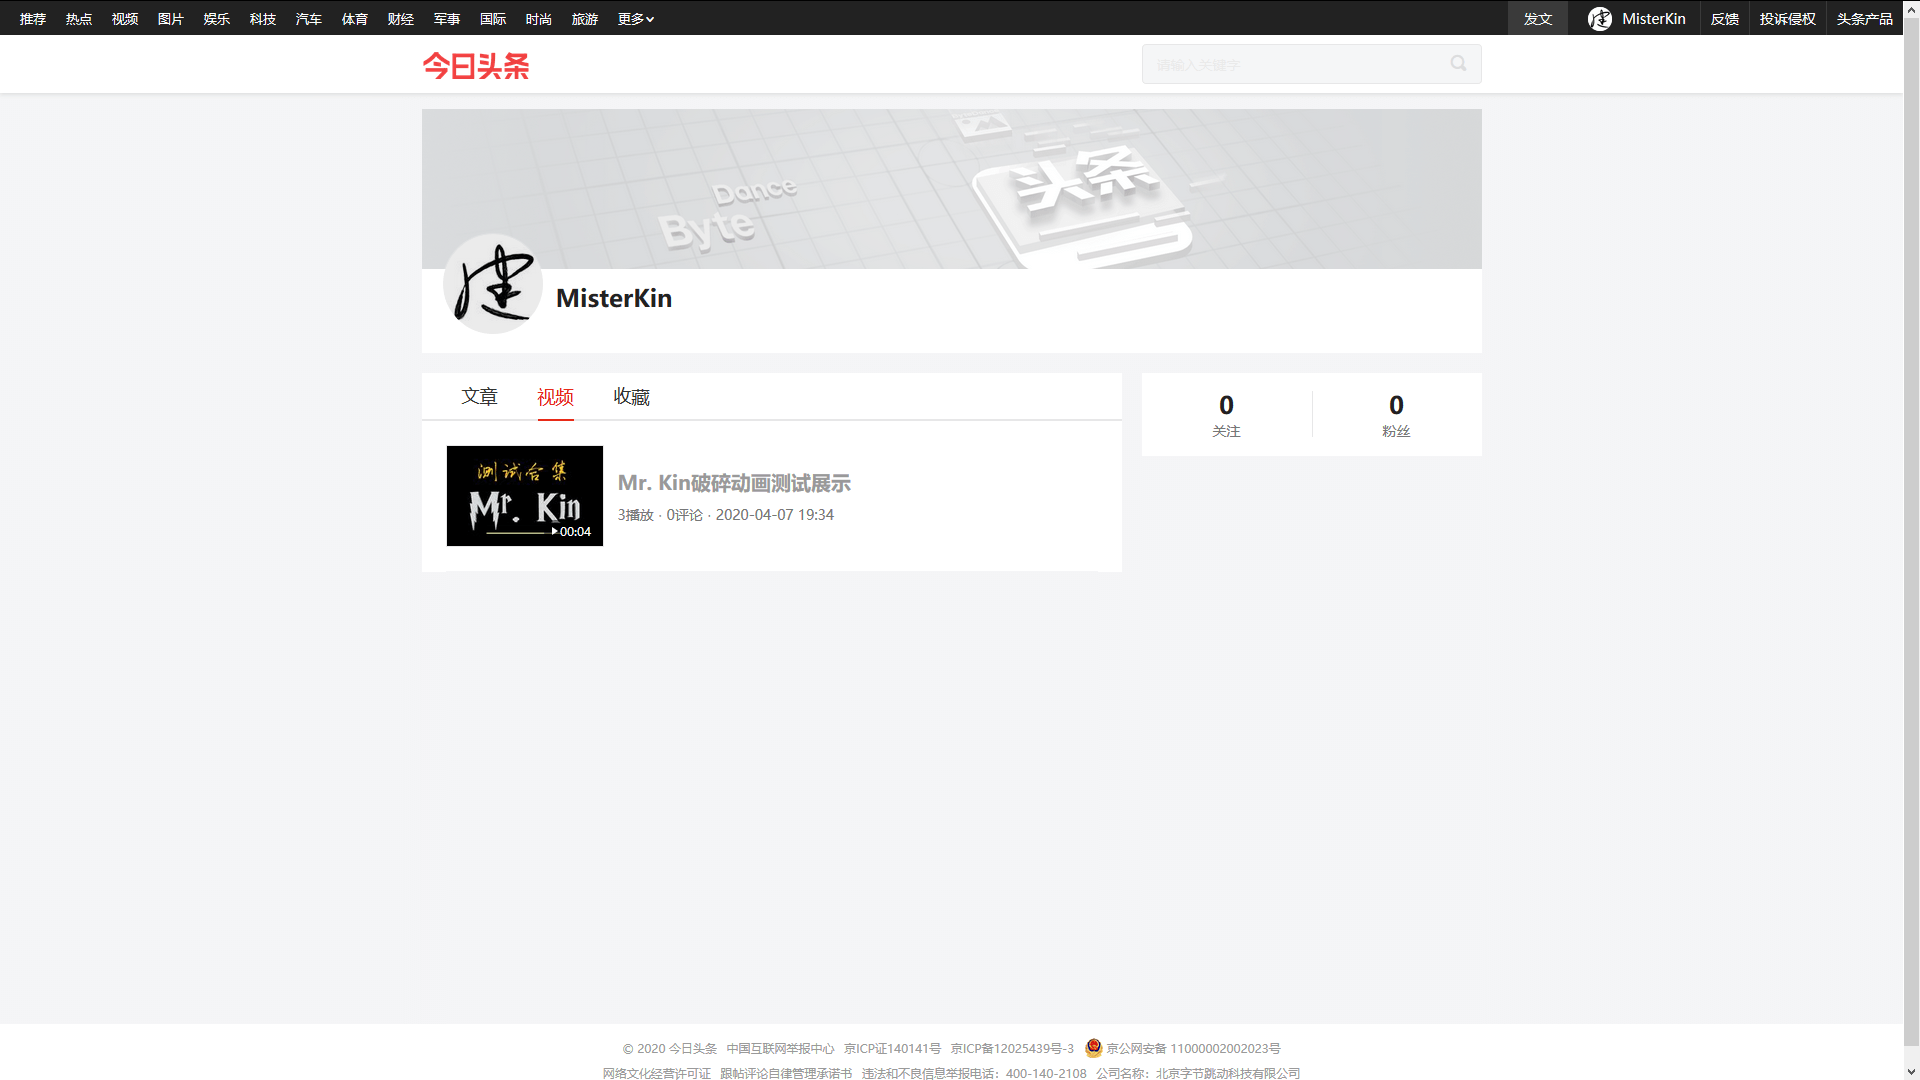
\includegraphics[scale=0.055]{Headline}
        \end{minipage}
        \qquad
        \begin{minipage}[t]{0.2\textwidth}
            \centering
            \setlength{\abovecaptionskip}{1pt}
            \setlength{\belowcaptionskip}{10pt}
            \caption*{\href{https://www.youtube.com/channel/UCNhtdG6whC5mlRDkrhQ0wLA?view_as=public}{油管 - Youtube}}
            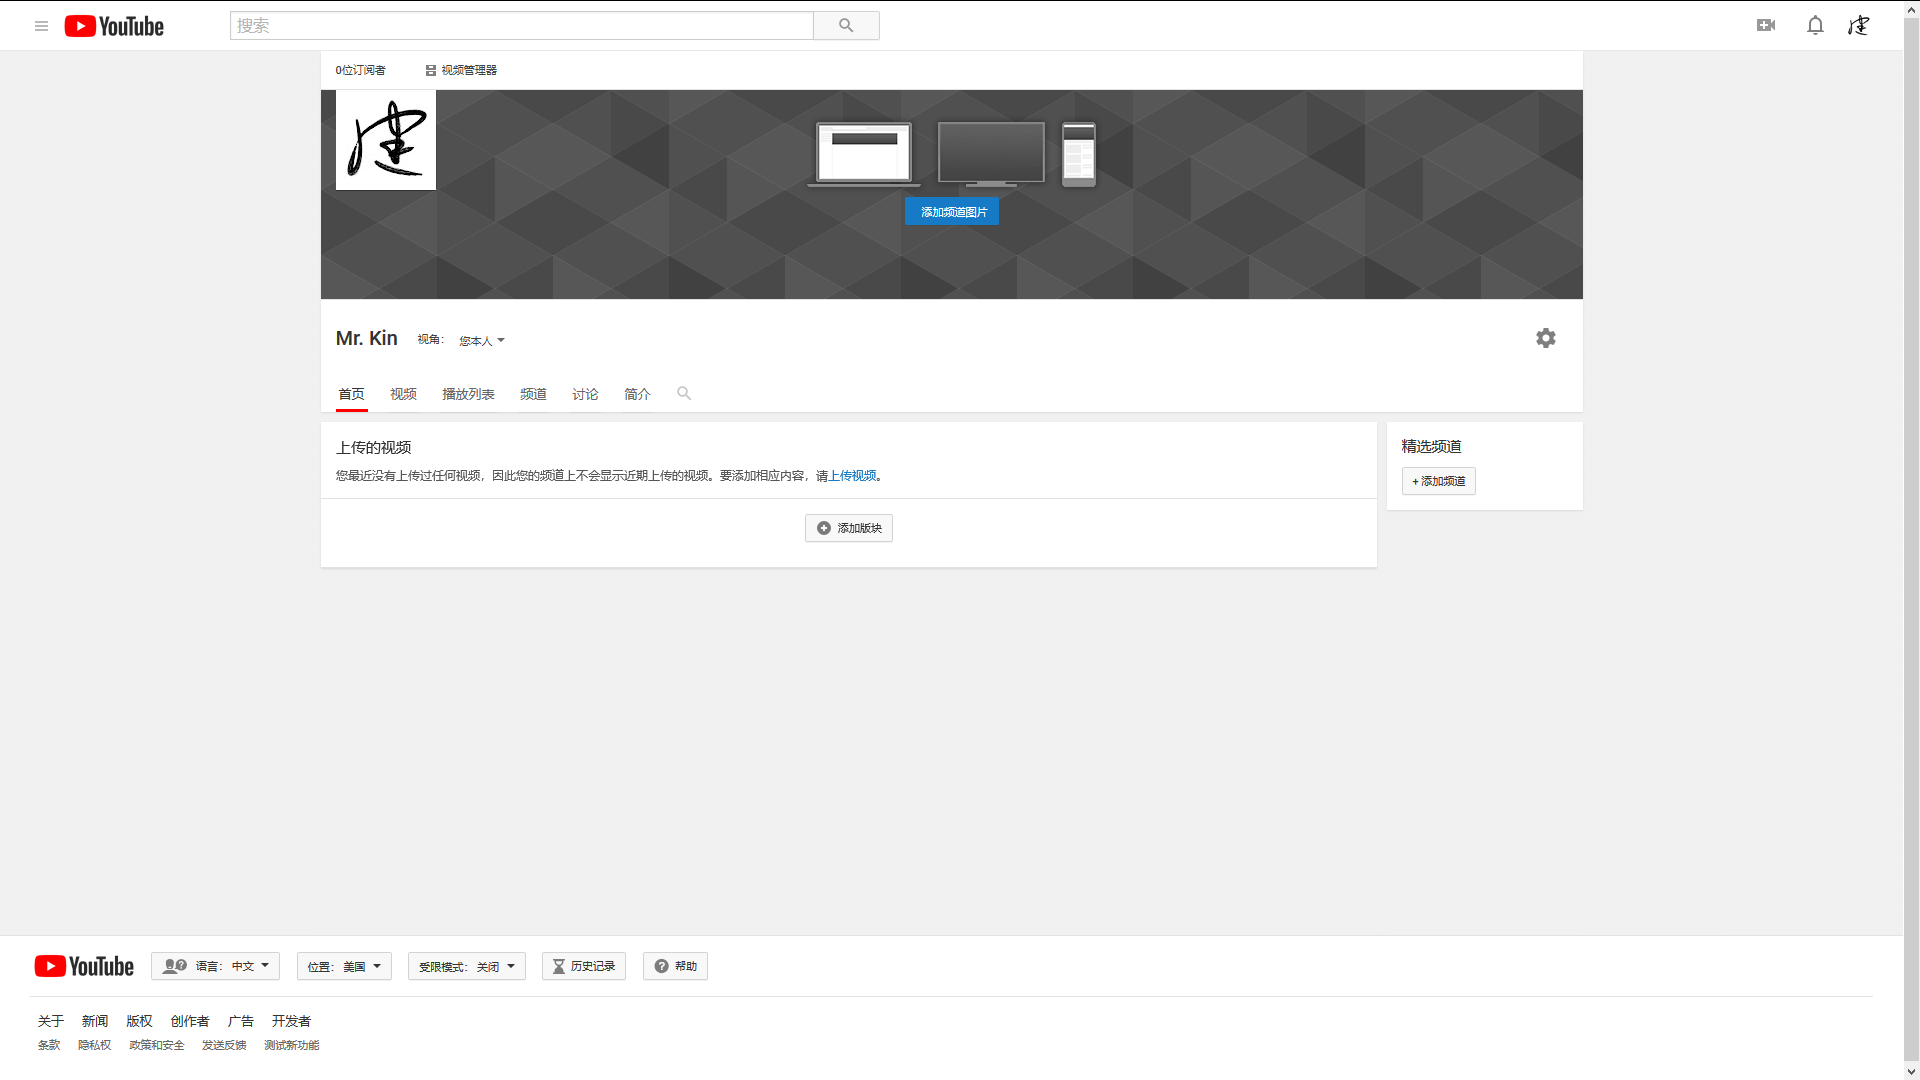
\includegraphics[scale=0.055]{Youtube}
        \end{minipage}
        \qquad
    \end{figure}

    \ifx\collections\undefined
    \printbibliography %生成参考文献排版。
    \addcontentsline{toc}{section}{参考文献} %添加参考文献进目录
    \clearpage %新建页,确保超链接跳转正确
    \phantomsection %确保目录中的超链接指向正确的页码
    \printindex %生成索引排版。
\end{document}
    \fi
 %关于页面
    \phantomsection
\begin{center}
    {\bfseries\sffamily\Large 版权声明}
\end{center}
\addcontentsline{toc}{chapter}{版权声明}

\noindent 作者:Mr. Kin \\
\DetectToksEmpty\LinkBlogPost
\ifToksEmpty
博文链接:链接暂空\\
\else
博文链接:\href{\the\LinkBlogPost}{跳转博文页}\\
\fi
\DetectToksEmpty\LinkPDFSource
\ifToksEmpty
PDF及LaTex源码链接:链接暂空\\
\else
PDF及LaTex源码链接:\href{\the\LinkPDFSource}{跳转PDF及LaTex源码页}\\
\fi
\DetectToksEmpty\LinkVideo
\ifToksEmpty
\else
相关视频创作链接:\href{\the\LinkVideo}{跳转视频页}\\
\fi
许可协议:本作品的所有内容,除个人设计创作的图像(如logo等)和相关的视频创作及其他特别声明外,均采用\href{https://creativecommons.org/licenses/by-nc-sa/4.0/deed.zh}{知识共享\ 署名-非商业性使用-相同方式共享 4.0 国际许可协议}进行发布。版权 © Mr. Kin,保留所有权利。
\includegraphics[scale=.4]{CC-BY-NC-SA}\\*[1.3ex]
\begin{tabular}{|*{3}{p{0.306\textwidth}|}}
    \hline
    \textsf{\bfseries 允许} & \textsf{\bfseries 限制} & \textsf{\bfseries 条件} \\
    \hline
    \vspace{-8pt}{\color{green}√} 修改 & \vspace{-8pt}{\color{red}×} 商标使用 & \vspace{-8pt}{\color{blue}$\odot$} 保留原署名 \\[-12pt]
    {\color{green}√} 分发 & {\color{red}×} 专利使用 & {\color{blue}$\odot$} 状态变更说明 \\[-12pt]
    {\color{green}√} 个人使用 & {\color{red}×} 商业使用 & {\color{blue}$\odot$} 相同的许可和版权声明 \\
    \hline
\end{tabular}
\\*[1.3ex]
\emph{注:若想对本作品进行转载、引用亦或是进行二次创作时,请详细阅读上述相关协议内容(若不理解,请点击链接跳转阅读)。为保障本人权利,对于违反者,本人将依法予以处理!望周知!——Mr. Kin}

\begin{center}
    {\bfseries\sffamily\Large 勘误声明}
\end{center}

虽本人写作时已尽力保证其内容的正确性,但因个人知识面和经验的局限性以及计算机技术等相关技术日新月异,本作品内容或存在一些错误之处。还望诸君发现错误后能够\hyperlink{contact}{联系我}以更正错误,不胜感激!——Mr. Kin

\begin{center}
    {\bfseries\sffamily\Large 侵权声明}
\end{center}

若本作品采用的第三方内容侵犯了你的版权,请与我\hyperlink{contact}{联系}进行处理,谢谢!——Mr. Kin

\begin{center}
    {\bfseries\sffamily\Large 第三方开源许可声明}
\end{center}

\noindent 本作品使用的第三方开源产品有:
\begin{multicols}{2}
\begin{itemize}
    \item \href{https://github.com/adobe-fonts}{Adobe Fonts}: \href{https://github.com/adobe-fonts/source-serif-pro/blob/release/LICENSE.md}{OFL v1.1}
    \item \href{https://tug.org/texlive/}{Tex Live}: \href{https://tug.org/texlive/copying.html}{TeX Live Licensing}
    \item \href{https://code.visualstudio.com/}{Visual Studio Code}: \href{https://github.com/Microsoft/vscode/blob/master/LICENSE.txt}{MIT}
    \item \href{http://ffmpeg.org/}{FFmpeg}: \href{http://ffmpeg.org/legal.html}{LGPL v2.1 / GPL v2}
    \item \href{https://krita.org/en/}{Krita}: \href{https://docs.krita.org/en/KritaFAQ.html?highlight=license#license-rights-and-the-krita-foundation}{Krita's GPL license}
    \item \href{https://inkscape.org/}{Inkscape}: \href{https://inkscape.org/about/license/}{GPL}
    \item \href{https://www.gimp.org}{GIMP}: \href{https://www.gimp.org/about/COPYING}{GPL}
    \item \href{https://www.blender.org}{Blender}: \href{https://www.blender.org/about/license/}{GPL}
    \item \href{https://www.audacityteam.org/}{Audacity}: \href{https://www.audacityteam.org/about/license/}{GPL v2}
    \item \href{https://handbrake.fr}{Handbrake}: \href{https://github.com/HandBrake/HandBrake/blob/master/LICENSE}{GPL v2}
\end{itemize}
\end{multicols}

\noindent 更多请点击查看\href{https://mister-kin.github.io/about/third-party-declaration/}{第三方声明页}!
 %版权声明
    {\centering \tableofcontents} %生成目录页
    \clearpage %新建页,分离上下两个样式页码的效果
    \pagenumbering{arabic} %阿拉伯样式页码

    % !TEX root = English.tex %指定主文件
\ifx\collections\undefined
% !TEX program = xelatex %指定编译方式xelatex。
% !BIB program = biber %指定bib数据后台处理程序biber。
\documentclass[11pt,a4paper,UTF8,titlepage]{ctexrep} %指定ctex的文档类,设置基本字号为11pt,a4大小,使用UTF-8编码保存,指定\maketitle生成单独的标题页。

\usepackage{syntonly}
%\syntaxonly %用来快速编译以排查错误,不生成DVI或PDF。
\usepackage[style=gb7714-2015]{biblatex} %调用biblatex宏包,设置参考文献样式(符合中文文献著录标准GB/T 7714-2015的样式),使用默认的后端程序biber(其支持更好,包括UTF-8等)放弃使用[backend=bibtex](只支持ascii编码)。
\addbibresource{resources/reference.bib} %加载参考文献数据库。
\usepackage{makeidx}
\makeindex %开启索引收集
\usepackage[margin=1in]{geometry} %调用geometry宏包,设置周围页边距为1英寸(为电子档设计,非打印)。
\usepackage{xcolor} %调用xcolor宏包,以支持扩展生成颜色。
\usepackage{fontspec} %调用fontspec宏包以更改西文字体族。
\setmainfont{Source Serif Pro}
\setsansfont{Source Sans Pro}
\setmonofont{Source Code Pro}
\usepackage{xeCJK} %调用xeCJK宏包以更改中文字体族。
\xeCJKsetup{AutoFakeSlant=true}  %设置xeCJK选项-伪斜体(需置于字体设置之前)。
\setCJKmainfont{思源宋体}
\setCJKsansfont{思源黑体}
\setCJKmonofont{思源等宽}
\usepackage{graphicx} %调用graphicx宏包,以支持插图。
\graphicspath{{resources/images/},{resources/images/follow/}} %加载图片路径。
\usepackage{caption} %调用caption,支持不带编号的标题。
\usepackage{wrapfig} %调用wrapfig,支持图文排版。
\usepackage{subfigure} %调用subfigure宏包进行图片图片排版。
\usepackage{tikz,tikz-qtree} %调用tikz及其扩展宏包,以支持画图。
\usepackage[subfigure]{tocloft} %tocloft与subfigure宏包冲突,不能简单调用,tocloft需设置参数。
\usepackage{tocbibind} %调用宏包以添加目录本身和参考文献进目录中。
\usepackage{multicol} %调用multicol宏包以支持多栏排版。
\usepackage[toc]{multitoc} %调用multitoc宏包,设置toc目录页,默认双栏排版。
\usepackage{enumitem} %调用emuitem,以设置列表环境。
\usepackage{multirow} %调用multirow,以支持纵向合并列表。
%重订制目录命令。
\renewcommand{\tableofcontents}%
  {\chapter{\contentsname}%
  \@mkboth{\MakeUppercase\contentsname}{\MakeUppercase\contentsname}%
  \@makeschapterhead{\sourcecodename}%
  \@starttoc{toc}%
}
\usepackage{fancyhdr} %调用宏包,以设置页眉,统一格式:标题在左,页码在右。
\pagestyle{fancy}
\fancyhf{}
\fancyhead[LO]{\sffamily \rightmark}
\fancyhead[LE]{\sffamily \leftmark}
\fancyhead[ROE]{\bfseries \thepage}
\fancyfoot[COE]{\ttfamily \href{https://mister-kin.github.io}{个人博客:https://mister-kin.github.io}}
%定义intro环境。
\newenvironment{intro}{\narrower\sffamily}{\par\vspace*{2ex plus 2.5ex minus 1.5ex}}
\usepackage{listings} % 指定listings,订制代码排版环境
\lstset{
    basicstyle      = \ttfamily,                          % 基本代码指定等宽字体
    keywordstyle    = \bfseries,                          % 关键字指定加粗
    commentstyle    = \ttfamily\slshape\color{gray},      % 注释指定灰色等宽斜体
    stringstyle     = \ttfamily,                          % 字符串指定等宽字体
    %numbers        = left,                               % 行号的位置在左边,启用后不方便复制代码
    %numberstyle    = \ttfamily,                          % 行号等宽字体
    %xleftmargin    = \parindent,                         % 代码左边框起始位置(启用行号时建议启用这个)
    %frame          = trBL,                               % 代码框类型,t下,r右,b下,l左,大写时为两条线。
    %frameround     = fttt,                               % 控制代码框是否为圆角
    frameshape      = {{ryrynyyyy}{yny}{yny}{ryrynyyyy}}, % 控制边框样式,上下边是每三个字母段控制一条边框。
    backgroundcolor = \color{gray!5},                     % 代码框背景颜色:5%的灰色
    breaklines      = true,                               % 代码过长时则换行
    gobble          = 8,                                  % 去掉代码前的缩进
}
\usepackage{hyperref} %调用hyperref宏包
\hypersetup{
    colorlinks=true, %设置超链接文件带颜色
    bookmarks=true, %生成书签
    bookmarksopen=true, %书签展开
    bookmarksnumbered=true, %书签带章节编号
    CJKbookmarks=true, %cjk必设参数
    unicode, %utf-8编码必设参数
    pdftitle=标题, %设置PDF文件属性标题
    pdfauthor=Mr. Kin, %设置PDF文件属性作者
    pdfstartview=FitH %默认适合宽度显示
}

    \title{\hypertarget{title}{\textbf{标题}}}
    \addcontentsline{toc}{chapter}{标题页}
    \author{Written by Mr. Kin}
    \date{创建于2020.1.28,修改于\number\year.\number\month.\number\day}

\begin{document}
    \phantomsection %确保目录中的超链接指向正确的页码
    \pdfbookmark[1]{标题页}{title} %添加标题页书签
    \pagenumbering{Roman} %大写罗马样式页码
    \maketitle %生成标题页
    \pagenumbering{roman} %小写罗马样式页码
    {\centering \tableofcontents} %生成目录页
    \clearpage %新建页,分离上下两个样式页码的效果
    \pagenumbering{arabic} %阿拉伯样式页码
    \fi

    \chapter*{词典常用缩写}
    \addcontentsline{toc}{chapter}{词典常用缩写}
    \markright{词典常用缩写}
    \begin{multicols}{2}
        \begin{itemize}[left=0em]
            \item v. verb 动词
            \item vt. transitive verb 及物动词
            \item vi. intransitive verb 不及物动词
            \item n. noun 名词
            \item adj. adjective 形容词
            \item adv. adverb 副词
            \item prep. preposition 介词
            \item pron. pronoun 代词
            \item conj. conjunction 连词
            \item abbr. abbreviation 缩写
            \item det. determiner 限定词
            \item sing. singular 单数
            \item pl. plural 复数
            \item symb. symbol 符号
            \item opp. opposite 反义词
            \item syn. synonym 同义词
            \item fig. figurative 比喻的
            \item derog. derogatie 贬义的
            \item fml. formal 用于正式文体
            \item infml. informal 用于非正式文体
            \item BrE 英国英语
            \item AmE 美国英语
            \item C countable 可数名词
            \item U uncountable 不可数名词
            \item sb. somebody 某人
            \item sth. something 某事物
            \item pt past tense 过去时
            \item pp past participle 过去分词
            \item \quad[计] 计算机
            \item \quad[物] 物理
            \item \quad[电] 电路
            \item \quad[医] 医学
        \end{itemize}
    \end{multicols}

    \ifx\collections\undefined
    \printbibliography %生成参考文献排版。
    \addcontentsline{toc}{chapter}{参考文献} %添加参考文献进目录
    \clearpage %新建页,确保超链接跳转正确
    \phantomsection %确保目录中的超链接指向正确的页码
    \printindex %生成索引排版。
\end{document}
    \fi

    \part{词汇量积累篇}
    % !TEX root = English.tex %指定主文件
\ifx\collections\undefined
% !TEX program = xelatex %指定编译方式xelatex。
% !BIB program = biber %指定bib数据后台处理程序biber。
\documentclass[11pt,a4paper,UTF8,titlepage]{ctexrep} %指定ctex的文档类,设置基本字号为11pt,a4大小,使用UTF-8编码保存,指定\maketitle生成单独的标题页。

\usepackage{syntonly}
%\syntaxonly %用来快速编译以排查错误,不生成DVI或PDF。
\usepackage[style=gb7714-2015]{biblatex} %调用biblatex宏包,设置参考文献样式(符合中文文献著录标准GB/T 7714-2015的样式),使用默认的后端程序biber(其支持更好,包括UTF-8等)放弃使用[backend=bibtex](只支持ascii编码)。
\addbibresource{resources/reference.bib} %加载参考文献数据库。
\usepackage{makeidx}
\makeindex %开启索引收集
\usepackage[margin=1in]{geometry} %调用geometry宏包,设置周围页边距为1英寸(为电子档设计,非打印)。
\usepackage{xcolor} %调用xcolor宏包,以支持扩展生成颜色。
\usepackage{fontspec} %调用fontspec宏包以更改西文字体族。
\setmainfont{Source Serif Pro}
\setsansfont{Source Sans Pro}
\setmonofont{Source Code Pro}
\usepackage{xeCJK} %调用xeCJK宏包以更改中文字体族。
\xeCJKsetup{AutoFakeSlant=true}  %设置xeCJK选项-伪斜体(需置于字体设置之前)。
\setCJKmainfont{思源宋体}
\setCJKsansfont{思源黑体}
\setCJKmonofont{思源等宽}
\usepackage{graphicx} %调用graphicx宏包,以支持插图。
\graphicspath{{resources/images/},{resources/images/FollowMe/}} %加载图片路径。
\usepackage{caption} %调用caption,支持不带编号的标题。
\usepackage{wrapfig} %调用wrapfig,支持图文排版。
\usepackage{subfigure} %调用subfigure宏包进行图片图片排版。
\usepackage{tikz,tikz-qtree} %调用tikz及其扩展宏包,以支持画图。
\usepackage[subfigure]{tocloft} %tocloft与subfigure宏包冲突,不能简单调用,tocloft需设置参数。
\usepackage{tocbibind} %调用宏包以添加目录本身和参考文献进目录中。
\usepackage{multicol} %调用multicol宏包以支持多栏排版。
\usepackage[toc]{multitoc} %调用multitoc宏包,设置toc目录页,默认双栏排版。
\usepackage{enumitem} %调用emuitem,以设置列表环境。
\usepackage{multirow} %调用multirow,以支持纵向合并列表。
\usepackage{ulem} %调用ulem,以支持删除线等。
%重订制目录命令。
\renewcommand{\tableofcontents}%
  {\chapter{\contentsname}%
  \@mkboth{\MakeUppercase\contentsname}{\MakeUppercase\contentsname}%
  \@makeschapterhead{\sourcecodename}%
  \@starttoc{toc}%
}
\usepackage{fancyhdr} %调用宏包,以设置页眉,统一格式:标题在左,页码在右。
\pagestyle{fancy}
\fancyhf{}
\fancyhead[LO]{\sffamily \rightmark}
\fancyhead[LE]{\sffamily \leftmark}
\fancyhead[ROE]{\bfseries \thepage}
\fancyfoot[COE]{\ttfamily \href{https://mister-kin.github.io}{个人博客:https://mister-kin.github.io}}
%定义intro环境。
\newenvironment{intro}{\narrower\sffamily}{\par\vspace*{2ex plus 2.5ex minus 1.5ex}}
\usepackage{listings} % 指定listings,订制代码排版环境
\lstset{
    basicstyle      = \ttfamily,                          % 基本代码指定等宽字体
    keywordstyle    = \bfseries,                          % 关键字指定加粗
    commentstyle    = \ttfamily\slshape\color{gray},      % 注释指定灰色等宽斜体
    stringstyle     = \ttfamily,                          % 字符串指定等宽字体
    %numbers        = left,                               % 行号的位置在左边,启用后不方便复制代码
    %numberstyle    = \ttfamily,                          % 行号等宽字体
    %xleftmargin    = \parindent,                         % 代码左边框起始位置(启用行号时建议启用这个)
    %frame          = trBL,                               % 代码框类型,t下,r右,b下,l左,大写时为两条线。
    %frameround     = fttt,                               % 控制代码框是否为圆角
    frameshape      = {{ryrynyyyy}{yny}{yny}{ryrynyyyy}}, % 控制边框样式,上下边是每三个字母段控制一条边框。
    backgroundcolor = \color{gray!5},                     % 代码框背景颜色:5%的灰色
    breaklines      = true,                               % 代码过长时则换行
    gobble          = 8,                                  % 去掉代码前的缩进
}
\usepackage{hyperref} %调用hyperref宏包
\hypersetup{
    colorlinks=true, %设置超链接文件带颜色
    bookmarks=true, %生成书签
    bookmarksopen=true, %书签展开
    bookmarksnumbered=true, %书签带章节编号
    CJKbookmarks=true, %cjk必设参数
    unicode, %utf-8编码必设参数
    pdftitle=标题, %设置PDF文件属性标题
    pdfauthor=Mr. Kin, %设置PDF文件属性作者
    pdfstartview=FitH %默认适合宽度显示
}

    \title{\hypertarget{title}{\textbf{标题}}}
    \addcontentsline{toc}{chapter}{标题页}
    \author{Written by Mr. Kin}
    \date{创建于2020.3.30,修改于\number\year.\number\month.\number\day}

\begin{document}
    \phantomsection %确保目录中的超链接指向正确的页码
    \pdfbookmark[1]{标题页}{title} %添加标题页书签
    \pagenumbering{Roman} %大写罗马样式页码
    \maketitle %生成标题页
    \pagenumbering{roman} %小写罗马样式页码
    {\centering \tableofcontents} %生成目录页
    \clearpage %新建页,分离上下两个样式页码的效果
    \pagenumbering{arabic} %阿拉伯样式页码
    \fi

    \chapter{软件}
    \section{Blender}
    \subsection{Video - BL 2.80 Fundamentals}
    \begin{multicols}{2}
        \begin{itemize}
            \item fantastic adj.极好的;很大的;怪诞的
            \item be mostly known for sth. 最出名的是……
            \item modeling capabilities 建模能力
            \item feature films 故事片
            \item TV series 电视连续剧
            \item a bunch of 一群;一束;一堆
            \item as of recently sth. 最近的……
            \item serve as 充当,担任
            \item an encyclopedia of sorts for fundamentals 各种基础的百科全书
            \item veteran adj.老手,经验丰富的
            \item intimidating adj.吓人的,令人胆怯的
            \item arguably adv.按理,可论证地
            \item handy adj.易使用的;便利的
            \item gizmo n.小装置,小玩意儿(个人理解为控件)
            \item axis n.轴,坐标轴,对称中心轴
            \item respond to 响应,作出反应
            \item indicator n.指针,指示器;指示信号,标志
            \item perspective adj.透视的 n.透视法;态度;客观判断力;景观
            \item orthographic adj.正交的
            \item corresponding adj.符合的,相关的
            \item achieve the same effect 达到相同效果
            \item pivot n.中心点,核心 v.使在枢轴上旋转
            \item particular adj.特指的;特别的
            \item point n.某地方,地点
            \item period n.句点;周期;一段时间
            \item number pad/numpad 数字键
            \item self-explanatory adj.无须解释的;一目了然的
            \item scroll n.卷轴 v.滚动
            \item plus n.加号;优势 adj.多,余;好的;零度以上 prep.加 conj.此外,况且
            \item minus n.减号 adj.负的 prep.减去;零下,欠缺
            \item go ahead 发生,进行;先走,走在前面
            \item take sth. into account/take account of sth. 考虑到,顾及
            \item flatten v.变平,把……弄平
            \item angle v.斜置,斜移
            \item immensely adv. 极端地,非常,极大地
            \item accurate adj.准确的
            \item in relation to (事物间)关系,关联(翻译常为「关于……」「在……方面」)
            \item flexible adj.灵活的,可变动的,柔韧的
            \item go over sth. 反复研究,仔细琢磨;仔细检查……
        \end{itemize}
    \end{multicols}


    \ifx\collections\undefined
    \printbibliography %生成参考文献排版。
    \addcontentsline{toc}{chapter}{参考文献} %添加参考文献进目录
    \clearpage %新建页,确保超链接跳转正确
    \phantomsection %确保目录中的超链接指向正确的页码
    \printindex %生成索引排版。
\end{document}
    \fi

    % !TEX root = EnglishVocabulary.tex %指定主文件
\ifx\collections\undefined
% !TEX program = xelatex %指定编译方式xelatex。
% !BIB program = biber %指定bib数据后台处理程序biber。
\documentclass[11pt,a4paper,UTF8,titlepage]{ctexart} %指定ctex的文档类,设置基本字号为11pt,a4大小,使用UTF-8编码保存,指定\maketitle生成单独的标题页。

\usepackage{syntonly}
%\syntaxonly %用来快速编译以排查错误,不生成DVI或PDF。
\usepackage[style=gb7714-2015]{biblatex} %调用biblatex宏包,设置参考文献样式(符合中文文献著录标准GB/T 7714-2015的样式),使用默认的后端程序biber(其支持更好,包括UTF-8等)放弃使用[backend=bibtex](只支持ascii编码)。
\addbibresource{resources/reference.bib} %加载参考文献数据库。
\usepackage{makeidx}
\makeindex %开启索引收集
\usepackage[margin=1in]{geometry} %调用geometry宏包,设置周围页边距为1英寸(为电子档设计,非打印)。
\usepackage{xcolor} %调用xcolor宏包,以支持扩展生成颜色。
\usepackage{fontspec} %调用fontspec宏包以更改西文字体族。
\setmainfont{Source Serif Pro}
\setsansfont{Source Sans Pro}
\setmonofont{Source Code Pro}
\usepackage{xeCJK} %调用xeCJK宏包以更改中文字体族。
\xeCJKsetup{AutoFakeSlant=true}  %设置xeCJK选项-伪斜体(需置于字体设置之前)。
\setCJKmainfont{思源宋体}
\setCJKsansfont{思源黑体}
\setCJKmonofont{思源等宽}
\usepackage{graphicx} %调用graphicx宏包,以支持插图。
\graphicspath{{resources/images/},{resources/images/follow/}} %加载图片路径。
\usepackage{caption} %调用caption,支持不带编号的标题。
\usepackage{wrapfig} %调用wrapfig,支持图文排版。
\usepackage{subfigure} %调用subfigure宏包进行图片图片排版。
\usepackage{tikz,tikz-qtree} %调用tikz及其扩展宏包,以支持画图。
\usepackage[subfigure]{tocloft} %tocloft与subfigure宏包冲突,不能简单调用,tocloft需设置参数。
\usepackage{tocbibind} %调用宏包以添加目录本身和参考文献进目录中。
\usepackage{multicol} %调用multicol宏包以支持多栏排版。
\usepackage[toc]{multitoc} %调用multitoc宏包,设置toc目录页,默认双栏排版。
\usepackage{enumitem} %调用emuitem,以设置列表环境。
%重订制目录命令。
\renewcommand{\tableofcontents}%
  {\chapter{\contentsname}%
  \@mkboth{\MakeUppercase\contentsname}{\MakeUppercase\contentsname}%
  \@makeschapterhead{\sourcecodename}%
  \@starttoc{toc}%
}
\usepackage{fancyhdr} %调用宏包,以设置页眉,统一格式:标题在左,页码在右。
\pagestyle{fancy}
\fancyhf{}
\fancyhead[LO]{\sffamily \rightmark}
\fancyhead[LE]{\sffamily \leftmark}
\fancyhead[ROE]{\bfseries \thepage}
%定义intro环境。
\newenvironment{intro}{\narrower\sffamily}{\par\vspace*{2ex plus 2.5ex minus 1.5ex}}
\usepackage{hyperref} %调用hyperref宏包
\hypersetup{
    colorlinks=true, %设置超链接文件带颜色
    bookmarks=true, %生成书签
    bookmarksopen=true, %书签展开
    bookmarksnumbered=true, %书签带章节编号
    CJKbookmarks=true, %cjk必设参数
    unicode, %utf-8编码必设参数
    pdftitle=标题, %设置PDF文件属性标题
    pdfauthor=Mr. Kin, %设置PDF文件属性作者
    pdfstartview=FitH %默认适合宽度显示
}

    \title{\hypertarget{title}{\textbf{标题}}}
    \addcontentsline{toc}{section}{标题页}
    \author{Written by Mr. Kin}
    \date{创建于2020.1.28,修改于\number\year.\number\month.\number\day}

\begin{document}
    \phantomsection %确保目录中的超链接指向正确的页码
    \pdfbookmark[1]{标题页}{title} %添加标题页书签
    \pagenumbering{Roman} %大写罗马样式页码
    \maketitle %生成标题页
    \pagenumbering{roman} %小写罗马样式页码
    {\centering \tableofcontents} %生成目录页
    \clearpage %新建页,分离上下两个样式页码的效果
    \pagenumbering{arabic} %阿拉伯样式页码
    \fi
    
    \section{IELTS雅思词汇圣经}
    \subsection{6分词汇}
    \subsubsection{list 1}
    \begin{multicols}{2}
    \begin{itemize}
        \item abstract adj.抽象的 n.摘要,概要\\thinking in abstract terms 抽象思维\\同 theoretical 反 concrete
        \item abundance n.大量,充足\\an abundance of sth. 大量的xx\\同 sufficiency 反lack
        \item abuse v.滥用,妄用;虐待(尤指性)n.滥用,虐待[U,pl.]\\abuse sb./sth. 虐待xx/滥用xx\\ abuse of power 滥用职权\\ child abuse 儿童虐待\\同 misapply, make ill use of; ill-treat
        \item baggage n.(AmE)行李 \\同 luggage
        \item candidate n.候选人,申请人(竞选/求职)\\candidate for sth. xx的候选人\\同 applicant, seeker
        \item canteen n.食堂,餐厅
        \item capable adj.有能力的,有才能的\\be capable of doing 有能力做xx\\同 able,competent 反 incapable
        \item capacity n.容量;能力\\a capacity of num+单位 有xx的容量\\同 ability
        \item capital n.资本,资金;首都;大写字母
        \item data n.资料,数据
        \item date n.日期,日子;年份 v.存在,追溯\\date back to medieval times 始于中世纪\\date back hundreds of years 追溯到几百年前\\date from the 17th century 自17世纪起
        \item economy n.经济
        \item edition n.版本(出版)\\同 version
        \item facilitate v.促进,促使,使便利\\同 ease
        \item facilities n.设施,设备\\sporting facilities 运动设施
        \item gamble v.赌博(用钱)\\gamble sth away 赌掉xx\\gamble on sth./on doing sth. 冒xx的风险/碰xx的运气\\同 bet, try one's luck
        \item gang n.一群,一伙(闹事青少年)
        \item hairdresser n.理发师
        \item identification n.身份证明\\同 recognition
        \item identify v.确认、证明\\identify sb./sth. 鉴别出xx\\identify sb. with sth. 把某人视为xx\\同 determine
        \item idiom n.习语,成语,惯用语
        \item idle adj.闲散的,无工作的 v.无所事事;闲荡\\idle sb./sth. (暂时性)关闭工厂,使工人闲着\\近 inactive,lazy 反 busy(adj./n.)\\idle和busy/load也常用于计算机
        \item jar n.广口瓶
        \item jealous adj.嫉羡的,羡慕的\\be jealous of sb./sth. 妒忌xx\\近 envious
        \item labour n.劳动,劳力 v.努力做(困难的事);干苦力活\\labour to do sth. 努力做xx\\近 work
        \item lack v.没有(某事物),缺乏,缺少,不足\\近 need(provide assistance in need 提供帮助)(need指缺乏,食物、钱、生活来源)
        \item magnify v.放大;夸张,夸大\\同 enlarge 反 minify
        \item naive adj.缺乏经验的,幼稚无知的;天真的\\同 innocent, simple
        \item overview n.(fml.)综览,概观,概述
        \item pension n.养老金,抚恤金,退休金
        \item perceive v.理解,认为;意识到,注意到\\同 detect
        \item percent n./adj.百分比
        \item percentage n.百分数;比例
        \item responsible adj.有责任的,承担义务的\\同 accountable
        \item restore v.回复(某种情况/感受)\\同 recover
        \item restrain v.制止,管制(武力)\\同 inhibit
        \item setback n.挫折,阻碍
        \item severe adj.严格的,苛刻的,纪律严明的
        \item shabby adj.因使用过久或管理不善而破旧
        \item shallow adj.浅的\\同 superficial 反 deep
        \item yield v.出产(作物),产生(效益)n.产量,产出,利润
        \item youngstar n.(infml.)年轻人,少年,儿童\\同 juvenile
    \end{itemize}
    \end{multicols}
    \subsubsection{list 2}
    \begin{multicols}{2}
        \begin{itemize}
            \item abandon v.离弃,舍弃\\同 desert,forsake 反reclaim
            \item abnormal adj.反常的,变态的\\反normal
            \item absorb v.吸收\\同give out
            \item bacteria n.(pl.)细菌\\sing. bacterium
            \item badminton n.羽毛球运动
            \item cafeteria n.自助餐厅,自助食堂\\同 coffee shop, lunchroom
            \item calculate v.计算,推算\\同 compute, estimate
            \item calendar n.日历,挂历\\同 programme
            \item campus n.校园,校区(大学、学院的)
            \item cancel v.取消,撤销\\同 drop, call off
            \item damage n./v.损失,损害,损毁\\同 ingury/ingure
            \item damp n.不完全干燥的,潮湿的\\反 dry
            \item dash v.猛冲,突进\\同 rush
            \item ease n.容易,不费劲\\反 burden
            \item ecology n.生态关系,生态学
            \item fabric n.织物,布料\\同 material
            \item fabulous adj.极好的,绝妙的\\同 wonderful
            \item gallery n.走廊,柱廊
            \item habitat n.自然环境(动/植物的),栖息地
            \item ideal adj.理想的,完美的;最合适的 n.完美的人或事物\\同 flawless,perfect
            \item idealism n.理想主义者,唯心论
        \end{itemize}
    \end{multicols}

    \ifx\collections\undefined
    \printbibliography %生成参考文献排版。
    \addcontentsline{toc}{section}{参考文献} %添加参考文献进目录
    \clearpage %新建页,确保超链接跳转正确
    \phantomsection %确保目录中的超链接指向正确的页码
    \printindex %生成索引排版。
\end{document}
    \fi
    % !TEX root = main.tex %指定主文件
\ifx\collections\undefined
% !TEX program = xelatex %指定编译方式xelatex。
% !BIB program = biber %指定bib数据后台处理程序biber。
\documentclass[11pt,a4paper,UTF8,titlepage]{ctexart} %指定ctex的文档类,设置基本字号为11pt,a4大小,使用UTF-8编码保存,指定\maketitle生成单独的标题页。

\usepackage{syntonly}
%\syntaxonly %用来快速编译以排查错误,不生成DVI或PDF。
\usepackage[style=gb7714-2015]{biblatex} %调用biblatex宏包,设置参考文献样式(符合中文文献著录标准GB/T 7714-2015的样式),使用默认的后端程序biber(其支持更好,包括UTF-8等)放弃使用[backend=bibtex](只支持ascii编码)。
\addbibresource{resources/reference.bib} %加载参考文献数据库。
\usepackage{makeidx}
\makeindex %开启索引收集
\usepackage[margin=1in]{geometry} %调用geometry宏包,设置周围页边距为1英寸(为电子档设计,非打印)。
\usepackage{xcolor} %调用xcolor宏包,以支持扩展生成颜色。
\usepackage{fontspec} %调用fontspec宏包以更改西文字体族。
\setmainfont{Source Serif Pro}
\setsansfont{Source Sans Pro}
\setmonofont{Source Code Pro}
\usepackage{xeCJK} %调用xeCJK宏包以更改中文字体族。
\xeCJKsetup{AutoFakeSlant=true}  %设置xeCJK选项-伪斜体(需置于字体设置之前)。
\setCJKmainfont{思源宋体}
\setCJKsansfont{思源黑体}
\setCJKmonofont{思源等宽}
\usepackage{graphicx} %调用graphicx宏包,以支持插图。
\graphicspath{{resources/images/},{resources/images/follow/}} %加载图片路径。
\usepackage{caption} %调用caption,支持不带编号的标题。
\usepackage{wrapfig} %调用wrapfig,支持图文排版。
\usepackage{subfigure} %调用subfigure宏包进行图片图片排版。
\usepackage{tikz,tikz-qtree} %调用tikz及其扩展宏包,以支持画图。
\usepackage[subfigure]{tocloft} %tocloft与subfigure宏包冲突,不能简单调用,tocloft需设置参数。
\usepackage{tocbibind} %调用宏包以添加目录本身和参考文献进目录中。
\usepackage{multicol} %调用multicol宏包以支持多栏排版。
\usepackage[toc]{multitoc} %调用multitoc宏包,设置toc目录页,默认双栏排版。
\usepackage{enumitem} %调用emuitem,以设置列表环境。
%重订制目录命令。
\renewcommand{\tableofcontents}%
  {\chapter{\contentsname}%
  \@mkboth{\MakeUppercase\contentsname}{\MakeUppercase\contentsname}%
  \@makeschapterhead{\sourcecodename}%
  \@starttoc{toc}%
}
\usepackage{fancyhdr} %调用宏包,以设置页眉,统一格式:标题在左,页码在右。
\pagestyle{fancy}
\fancyhf{}
\fancyhead[LO]{\sffamily \rightmark}
\fancyhead[LE]{\sffamily \leftmark}
\fancyhead[ROE]{\bfseries \thepage}
%定义intro环境。
\newenvironment{intro}{\narrower\sffamily}{\par\vspace*{2ex plus 2.5ex minus 1.5ex}}
\usepackage{hyperref} %调用hyperref宏包
\hypersetup{
    colorlinks=true, %设置超链接文件带颜色
    bookmarks=true, %生成书签
    bookmarksopen=true, %书签展开
    bookmarksnumbered=true, %书签带章节编号
    CJKbookmarks=true, %cjk必设参数
    unicode, %utf-8编码必设参数
    pdftitle=标题, %设置PDF文件属性标题
    pdfauthor=Mr. Kin, %设置PDF文件属性作者
    pdfstartview=FitH %默认适合宽度显示
}

    \title{\hypertarget{title}{\textbf{标题}}}
    \addcontentsline{toc}{section}{标题页}
    \author{Written by Mr. Kin}
    \date{创建于2020.1.28,修改于\number\year.\number\month.\number\day}

\begin{document}
    \phantomsection %确保目录中的超链接指向正确的页码
    \pdfbookmark[1]{标题页}{title} %添加标题页书签
    \pagenumbering{Roman} %大写罗马样式页码
    \maketitle %生成标题页
    \pagenumbering{roman} %小写罗马样式页码
    {\centering \tableofcontents} %生成目录页
    \clearpage %新建页,分离上下两个样式页码的效果
    \pagenumbering{arabic} %阿拉伯样式页码
    \fi

    \section{电力专业英语}
    \subsection{Fundamentals of Electronic Circuits}
    \subsubsection{Circuit Theory}
    \begin{multicols}{2}
        \begin{itemize}
            \item element n.成分,元件
            \item interconnect vt.使互相连接
            \item node n.节点
            \item branch n.树枝,分枝,分部,支流,支脉 v.出现分岐
            \item loop n.环,循环,线圈(绳),弯曲部分,回路,回线 vt.使成环,使成圈,以环相连 vi.打环,翻筋斗
            \item topology n.拓扑,布局,拓扑学
            \item configuration n.构造,结构,配置,外形
            \item terminal n.终点站,终端,接线端
            \item resistor n.[电]电阻器
            \item independent n.独立自主者,无党派者 adj.独立自主的,不受约束的
            \item series n.连续,系列,级数,串联
            \item parallel adj.平行的,相同的,类似的,并联的 n.平行线,平行面,相似物 v.相应,平行
            \item impedance n.[电/物]阻抗,[物]全电阻
            \item theorem n.定理,法则(数)
        \end{itemize}
    \end{multicols}

    \subsubsection{Analog and Digital Circuits}
    \begin{multicols}{2}
        \begin{itemize}
            \item analog n.(AmE)类似物;模拟 adj.(AmE)模拟的,指针式的\\analogue n./adj.(BrE)同上
            \item digital n.数字,数字式 adj.数字的,数位的
            \item thermometer n.温度计,体温计
            \item Fahrenheit n.华氏温度计 adj.华氏温度计的
            \item drum n.鼓,鼓声,鼓形圆筒 vt.打鼓奏 vi.击鼓,做鼓声
            \item discrete adj.不连续的,离散的
            \item original adj.最初的,原始的,独创的,新颖的 n.原物,原作
            \item remote adj.遥远的,偏僻的,细微的
            \item bulb n.鳞茎,球形物
            \item Morse code 莫尔斯电码
            \item pulse n.脉搏,脉冲
            \item buzzer n.蜂鸣器,信号手,嗡嗡作声的东西
            \item manipulate vt.(熟练地)操作,使用(机器),操纵(人或市场、市场),利用,应付
            \item destination n.目的地,[计]目的文件,目的单元格
            \item humidity n.湿气,潮湿,湿度
            \item comparator n.比较仪
            \item trigger vt.引发,引起,触发 vi.转义,换车 n.扳机
            \item sequence n.次序,顺序,序列
            \item parallel n.平行的,相同的,类似的,并联的 n.平行线,平行面,相似物 v.相应,平行
            \item serial adj.连续的,串行的,顺次
            \item decoder n.解码器
            \item reassemble vt.重新召集 vi.重新集合
        \end{itemize}
    \end{multicols}

    \subsubsection{Three-Phase Circuits}
    \begin{multicols}{2}
        \begin{itemize}
            \item transformer n.变压器
            \item single-phase 单相
            \item pulsate vi.脉动
            \item three-phase power 三相电源
            \item three-phase circiut 三相电路
            \item the parallelogram method 平行四边形法则
            \item wye connection 星形连接
            \item delta connection 三角形连接
            \item phase voltage 相电压
            \item line voltage 线电压
            \item confuse vt.使混乱,使更难于理解,使困窘,使困惑 vi.使糊涂
            \item voltmeter n.电压表
            \item ammeter n.电流表
            \item clamp-on ammeter 钳式安培表
        \end{itemize}
    \end{multicols}

    \subsubsection{Further Reading}

    \subsection{Power Electronics}
    \subsubsection{Introduction}
    \begin{multicols}{2}
        \begin{itemize}
            \item solid-state adj.固态的
            \item computation n.计算,估计
            \item integration n.结合,整合,一体化
            \item dynamic adj.动态的,充满活力的,不断变化的 n.动态,动力学,活力
            \item mercury-arc [医]汞弧 \\Mercury n.水星
            \item valve n.阀,真空管,活栓 vt.装阀(于),以活门调节
            \item semiconductor n.[物理]半导体
            \item switching n.开关,转换,交换,配电 v.转换
            \item diode n.二极管
            \item inverter n.逆变器(反用换流器),变极器
            \item thyristor n.半导体闸流管,硅可控整流器
            \item inverter thyristor 晶体管逆变器,可控硅环流器,可控硅逆变器
            \item transistor n.晶体管,晶体管收音机,半导体收音机
            \item transmission n.播送,传送,信息,传动装置
            \item substantial adj.结实的,牢固的,重大的 n.本质,重要材料
            \item fluorescent lamp ballast 荧光灯镇流器
            \item mercury n.水银,汞
            \item therminoic adj.[物]热电子的,热离子的
            \item HVDC transmission system 高压直流输电系统
            \item induction motor 感应电动机
            \item vacuum n.真空,空间 adj.真空的 vt.用真空吸尘器打扫
            \item dissipate v.驱散,使(云/雾/疑虑)消散
            \item rectifier n.纠正者,整顿者,整流器
            \item triggered adj.触发的
            \item thyratron n.[电]闸流管
            \item ignitron n.引燃管,放电管
            \item cycloconverter n.周波变换器,循环换流器,双向离子变频器
            \item traic n.[电]三端双向可控硅开关元件
            \item a scope of 一个范围
            \item spectrum n.谱,光谱,范围,系列,幅度
        \end{itemize}
    \end{multicols}

    \ifx\collections\undefined
    \printbibliography %生成参考文献排版。
    \addcontentsline{toc}{section}{参考文献} %添加参考文献进目录
    \clearpage %新建页,确保超链接跳转正确
    \phantomsection %确保目录中的超链接指向正确的页码
    \printindex %生成索引排版。
\end{document}
    \fi
    \part{语法篇}

    \nocite{*} %不使用cite也能生成参考文献
    \printbibliography %生成参考文献排版。
    \addcontentsline{toc}{chapter}{参考文献} %添加参考文献进目录
    \clearpage %新建页,确保超链接跳转正确
    \phantomsection %确保目录中的超链接指向正确的页码
    \printindex %生成索引排版。
\end{document}
